\section{Introduction}

\subsection{Objectives} 

\begin{itemize}
\item Learn basic facts about the Karel language and its history. 
\item Learn how Karel differs from other programming languages.
\item Learn what skills this course will teach you.
\end{itemize}

\subsection{Brief history}

The educational programming language Karel the Robot was introduced by Richard E. 
Pattis in his book {\em Karel The Robot: A Gentle Introduction to the Art of Programming} in 1981. 
Pattis first used the language in his courses at Stanford University, and nowadays Karel is used at 
countless schools in the world. The language is named after Karel \v{C}apek, a Czech writer 
who invented the word "robot" in his 1921 science fiction play R.U.R. (Rossum's Universal Robots).
Various implementations of the language can be downloaded from the web, as shown in Fig. 
\ref{fig:intro-111}.

\begin{figure}[!ht]
\begin{center}
\includegraphics[width=4.9cm]{img/intro-112.png}\ \ \ 
\includegraphics[width=4.9cm]{img/intro-113.png}\ \ \ 
\includegraphics[width=4.9cm]{img/intro-114.png}
\caption{Various implementations of Karel that can be found on the web.}
\vspace{-4mm}
\label{fig:intro-111}
\end{center}
\end{figure}
\noindent
The original Karel language was strongly influenced by Pascal, a popular
language of the 1980s. 
Since Pascal is no longer being used today, we refreshed 
the language and adjusted its syntax to be close to Python, a modern high-level 
dynamic programming language. Our changes made the language much easier
to use. For illustration, compare the original Karel program\\

\begin{bbox}
\begin{verbatim}
BEGINNING-OF-PROGRAM
 
DEFINE turnright AS
BEGIN
    turnleft
    turnleft
    turnleft
END
 
BEGINNING-OF-EXECUTION
    ITERATE 3 TIMES
    BEGIN
        turnright
        move
    END
    turnoff
END-OF-EXECUTION
 
END-OF-PROGRAM
\end{verbatim}
\end{bbox}
\vspace{6mm}

\noindent
with its exact NCLab's Karel equivalent\\

\begin{bbox}
\begin{Verbatim}[commandchars=\\\{\}]
\PY{k}{def} turnright
    \PY{k}{repeat} 3
        \PY{n+nf}{left}
 
\PY{k}{repeat} 3
    turnright
    \PY{n+nf}{go}
\end{Verbatim}
\end{bbox}
\vspace{6mm}

\noindent
In fact, NCLab's Karel has a built-in command {\tt right} for the
right turn, so the above program can be written using just three lines:\\

\begin{bbox}
\begin{Verbatim}[commandchars=\\\{\}]
\PY{k}{repeat} 3
    \PY{n+nf}{right}
    \PY{n+nf}{go}
\end{Verbatim}
\end{bbox}
\vspace{6mm}

\noindent
The command {\tt right} was not part of the original Karel language  and thus 
it was added after a very careful consideration. The main reason for adding it was that it made 
Karel more pleasant to watch as he moves through the maze. Without this command, any right turn 
took three left turns, and as a result, Karel resembled a raging tornado.
Of course, orthodox Karel fans can still define and use their own {\tt rightturn} 
command. We made a few additional cosmetic changes to the language in order to make 
it more accessible to kids -- for example, beepers were replaced with gems, Karel 
has a home in the maze, and longer commands were replaced with simpler ones, such as 
{\tt leftturn} with {\tt left}, {\tt move} with {\tt go}, 
{\tt pickbeeper} with {\tt get} and {\tt putbeeper} with {\tt put}. 

NCLab's Karel has a Manual mode and three Programming modes. Programming 
modes 1 and 2 exactly correspond to the original Pattis' book. Programming mode 3 
introduces variables, lists, functions returning values, randomness, 
and a GPS device for the robot. As a result, Karel can do much more in Programming 
mode 3. In the rest of this textbook, when we say "Karel" we always mean "NCLab's Karel".

\subsection{Who is Karel?}

Karel is a little robot that lives in a maze and loves to collect gems.
He was manufactured with only five simple commands in his memory:

\begin{itemize}
\item {\color{blue} \tt go} ... make one step forward.
\item {\color{blue} \tt get} ... pick up a gem from the ground. 
\item {\color{blue} \tt left} ... turn to the left.
\item {\color{blue} \tt right} ... turn to the right. 
\item {\color{blue} \tt put} ... put a gem on the ground. 
\end{itemize}
He also has five built-in sensors that allow him to check his immediate surroundings:
\begin{itemize}
\item {\color{ForestGreen} \tt wall} ... helps the robot detect that a wall is right ahead.
\item {\color{ForestGreen} \tt gem} ... helps the robot detect that a gem lies under him.
\item {\color{ForestGreen} \tt north} ... helps the robot detect that he is facing North.
\item {\color{ForestGreen} \tt home} ... helps the robot detect that he is at home.
\item {\color{ForestGreen} \tt empty} ... helps the robot detect that his bag with gems is empty.
\end{itemize}

\subsection{What will this course teach you?}

Computer programming skills are highly valued today, and they will be even more 
valued in the future. Karel is the perfect language for beginners. It will teach
you how to design algorithms and write working computer programs without struggling 
with technical complications of mainstream programming languages. Thanks to its 
simplicity, you should be done with Karel fairly quickly, and in no time you will be 
ready to move on to other programming languages. In particular, NCLab offers
Python programming: Textbook with exercises and review questions is available in
the Help section of the Python module.  

\subsection{Is Karel a toy language?}

Not at all! Despite its playful appearance, Karel features all key
concepts of modern procedural programming. Computer programming includes two 
fairly independent tasks -- first to {\em design an algorithm} (sequence of 
steps leading to the solution of the problem at hand), and second, to {\em translate 
the algorithm into a suitable programming language}. The former skill is by 
far more important and therefore Karel puts maximum emphasis on it. This is 
why the language itself is kept so simple. As a matter of fact, the complexity 
of algorithms that you will encounter in this textbook ranges from trivial  
to extremely tough. Towards the end of the course you will encounter exercises
which you will probably not call toy problems.

\subsection{How does Karel differ from other programming languages?}

The biggest conceptual difference between Karel and mainstream procedural
programming languages such as Python, C, C++, Java or Fortran is that {\em 
the robot does not know math}. Math is present neither in Manual mode nor 
in Programming modes 1 and 2 that correspond to the Pattis' book. 
Math (except for logic) is not needed to understand how to design great 
algorithms and to translate them into efficient computer programs. 
 
\section{Launching Karel}

\subsection{Objectives} 
\begin{itemize}
\item Learn to launch Karel and work with the graphical application.
\item Learn that Karel has several modes and how they differ.
\end{itemize}
\noindent
The simplest way to launch Karel is to double click on the Programming icon on Desktop 
and select Karel in the menu. This will launch the application in Programming 
mode 1 with a demo program, as shown in Fig. 
\ref{fig:init}.

The demo program can be run by clicking on the green arrow button, and 
if no longer needed, it can be turned off in Settings. The demo script 
can be also erased by clicking on the "Clear cell" button under the cell.

\newpage

\begin{figure}[!ht]
\begin{center}
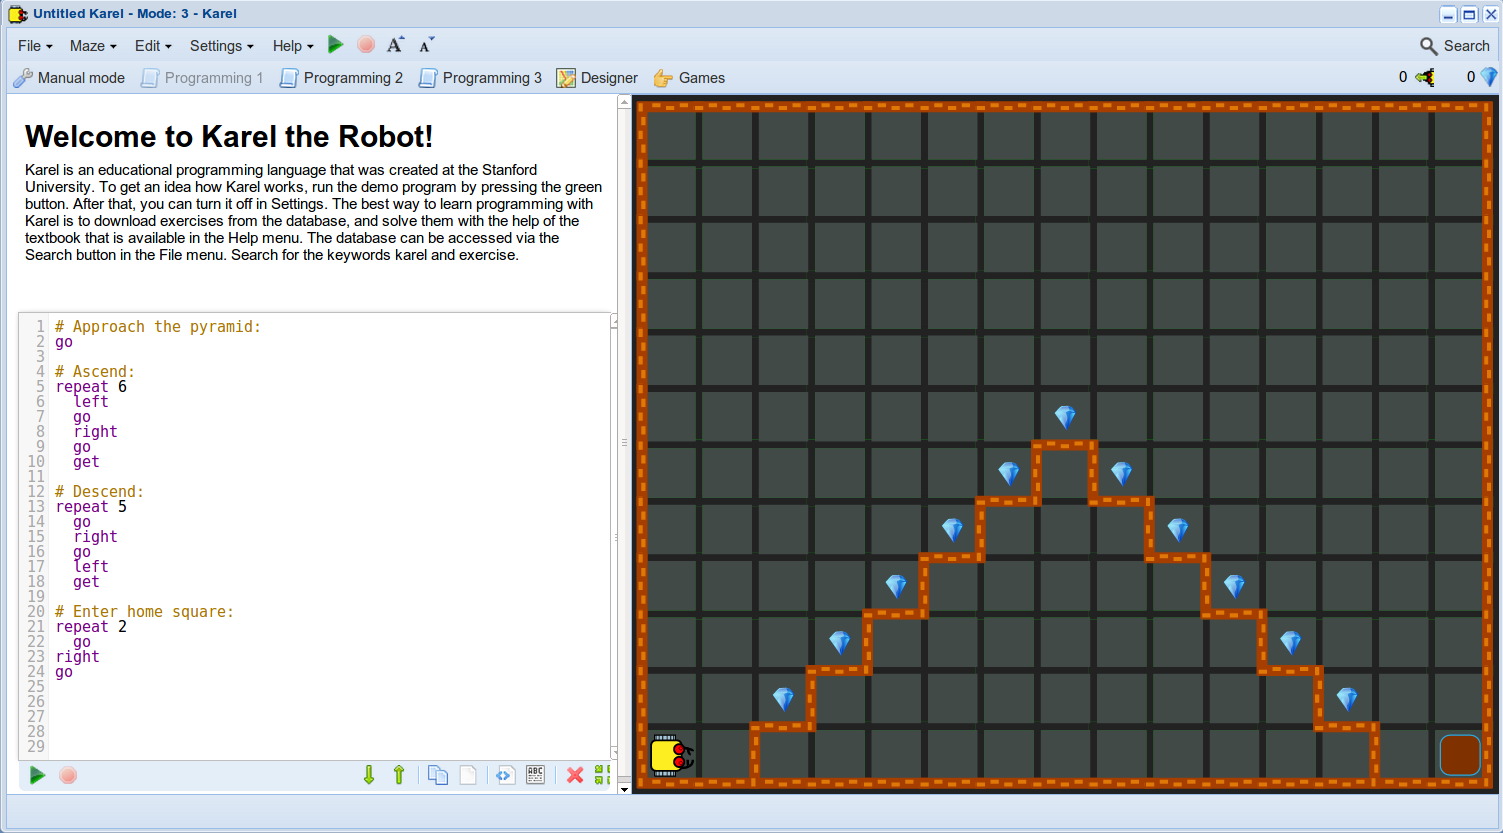
\includegraphics[width=0.7\textwidth]{img/init.png}
\end{center}
\vspace{-2mm}
\caption{Launching Karel in Programming mode 1, with a demo program.}
\label{fig:init}
%\vspace{-10mm}
\end{figure}

\noindent
From Programming mode 1, one can switch to Programming modes 2 and 3,
Manual mode, Designer mode, and Game mode. These modes will be discussed 
in more detail in Paragraph \ref{modes}.

The application window contains the main menu on top,
work area on the left, maze on the right, and status bar on the bottom.
The menus are fairly intuitive, so let us explain just a few selected 
functions. In the {\em File} menu:

\begin{itemize}
\item {\em Open} will open an existing Karel file.
\item {\em Search database} makes it possible to download Karel files from NCLab's
      public database to your NCLab account. In the Search box that appears, enter 
      keywords that best match what you are interested in. For example, typing 
      "karel textbook" will find all textbook exercises.  
\item {\em Publish to the web} will create a HTML address for your project. Such 
      a link can be included in any web page. 
\end{itemize}
The {\em Maze} menu facilitates operating with mazes, including creating a new random 
one, duplicating an existing maze, restoring maze to its saved version, and save and remove 
maze. The {\em Edit} menu enables operation with code cells and HTML cells (to be discussed in 
Section \ref{sec:editmenu}). In {\em Settings} one can change Karel's speed, adjust sound 
preferences, etc.

The green and red 
buttons are used to run and stop programs, respectively, and the two buttons next to them on
the right can be used to increase and decrease font size. The pair of icons on far right is the 
step counter (that can be reset by clicking on it) and gem counter that indicates how many gems 
Karel has in his bag.

\subsection{Karel modes} \label{modes}

Karel operates in six modes:
\begin{itemize}
\item {\em Manual mode.} The robot is controlled using the mouse and five buttons Go, Get, Left, Right, and Put. 
      Watch out and do not crash!
\item {\em Programming mode 1.} This mode serves 
      as a bridge between a world where the robot is guided via clicking on buttons, and another 
      world where he obeys written instructions. Programs are written using 
      six commands {\tt go}, {\tt get}, {\tt left}, {\tt right}, {\tt put}, and {\tt repeat}. The
      function of the former five corresponds exactly to the function of the buttons Go, Get, Left, 
      Right, and Put in Manual mode. The {\tt repeat} command will repeat a given number of times 
      any of the five basic commands, or their sequences, and it can also repeat other {\tt repeat} commands. 
\item {\em Programming mode 2.} This is where the actual programming begins. On top of the commands 
      from Programming mode 1, programs can contain conditions, conditional loops, and custom commands.
\item {\em Programming mode 3.} This mode goes beyond the original Pattis' book by introducing variables, 
      lists, random decisions, basic integer arithmetic, and functions that 
      return values. In this mode, Karel also gets a GPS device that allows him to determine his position 
      in the maze. 
\item {\em Designer mode} allows the user to create custom mazes.
\item {\em Game mode} makes it possible to create and play games. 
\end{itemize}

%%%%%%%%%%%%%%%%%%%%%%%%%%%%%%%%%%%%%%%%%%%%%%%%%%%%%%%%%%%%%%%%%%%%%%%%%%%%%%%

\section{Manual Mode} \label{sec:manual}

\subsection{Objectives} 
\begin{itemize}
\item Learn to guide the robot by clicking on buttons whose function corresponds to elementary commands.
\item Learn to work with spatial directions ``right'' and ``left'' relatively to the robot's orientation. 
\item Learn to plan your path ahead of time, and think before making a move.
\end{itemize}

\subsection{Compass}

Before we begin, let us review the four directions on the compass:
\newpage

\begin{figure}[!ht]
\begin{center}
\includegraphics[width=0.35\textwidth]{img/compass.png}
\vspace{-0mm}
%\caption{Karel's four possible orientations.}
%\label{fig:ori}
\end{center}
\vspace{-1cm}
\end{figure}

\subsection{Control buttons}

When launching Karel through the Programming icon, switch to Manual mode using the corresponding 
menu button. Then, five buttons Left, Right, Go, Get and Put will appear in the panel on the left,
as shown in Fig. \ref{fig:buttons}.

\begin{figure}[!ht]
\begin{center}
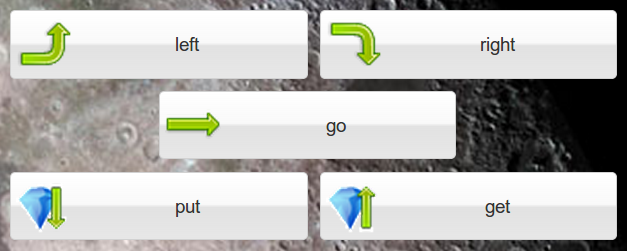
\includegraphics[width=6.2cm]{img/buttons-all.png}
\vspace{-0mm}
\caption{Karel's buttons in Manual mode (robot facing East).}
%\vspace{-1cm}
\label{fig:buttons}
\end{center}
\end{figure}
\noindent
The function of the buttons is self-explanatory -- pressing Left will turn the robot 90 degrees to the left,
pressing Right will turn him 90 degrees to the right, and pressing Go will move him one step forward. 
Upon pressing Put the robot will reach into his bag with gems, 
take one, and put it on the ground where he stands. 
An indicator showing how many gems are in the bag can be found in the upper right 
corner of the window. Last, upon pressing 
Get the robot will pick up a gem from the ground where he stands. If 
one asks the robot to get a gem where there is none, he will complain.

When the robot turns, the arrows on the buttons adjust automatically to his new 
direction. This is illustrated in Fig. \ref{fig:buttons2}.

\begin{figure}[!ht]
\begin{center}
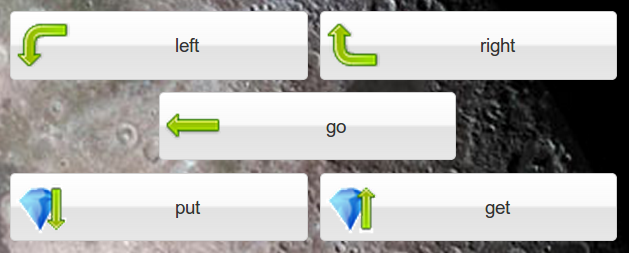
\includegraphics[width=6.2cm]{img/buttons-all-2.png}
\vspace{-0mm}
\caption{Karel's buttons in Manual mode (robot facing West).}
\label{fig:buttons2}
\end{center}
\end{figure}

%%%%%%%%%%%%%%%%%%%%%%%%%%%%%%%%%%%%%%%%%%%%%%%%%%%%%%%%%%%%%%%%%%%%%%%%%%%%%%%

\section{Programming Modes} \label{sec:bridge}

\subsection{Objectives} 
 
\begin{itemize}
\item Start programming!
\item Understand the difference between {\em algorithm} and {\em program}. 
\item Learn the difference between {\em logical} and {\em syntax} errors.
\item Understand that {\em debugging} is an indivisible part of computer programming.
\end{itemize}

\subsection{Typing programs}

Programs for the robot are entered into a {\em code cell} located on the left.
In Programming mode 1, we can use the commands {\tt left}, {\tt right}, {\tt go}, {\tt get}, 
{\tt put}, and {\tt repeat}.
The function of the former five is the same as the function of the corresponding buttons 
in Manual mode. One or more commands form {\em computer program (computer code)}. Often 
we just say {\em program} or {\em code}. There are two simple rules to remember:\\

\begin{gbox}
\begin{enumerate}
\item Always type one command per line, it greatly adds to code readability.
\item Indentation matters - do not enter any extra empty characters in front of commands. 
\end{enumerate}
\end{gbox}
\vspace{6mm}

\noindent
Ignoring these rules would not necessarily make your program invalid, 
but the code would be difficult to read. It is very important to write 
a clean, well readable code. 

\subsection{Algorithm} \label{subsec:interm1}

Karel always follows your commands {\em precisely}. No exceptions. Sometimes
the robot will do something that you will not expect. In this case most likely your 
{\em algorithm} was wrong. An {\em algorithm} is a sequence of 
steps (operations) that the robot follows in order to fulfill his task. Algorithms 
are written using normal human language, not in terms of computer code. Consider
a maze shown in Fig. \ref{fig:algo-1} where Karel needs to pick up the gem and 
return to his home square.

\begin{figure}[!ht]
\begin{center}
\includegraphics[width=6.6cm]{img/algo-1.png}
\vspace{-0mm}
\caption{Collect the gem and get home!}
\label{fig:algo-1}
%\vspace{-1.5cm}
\end{center}
\end{figure}
\noindent
An algorithm to solve this task would be:

\begin{verbatim}
Make two steps forward
Collect the gem and turn around
Make three steps forward
\end{verbatim}

\subsection{Program}

{\em Computer program} or just {\em program} is created by translating an algorithm 
to a particular programming language -- in our case to the Karel language. It is 
extremely important to have a good algorithm. Writing a program based on a good
algorithm is a routine. But if the algorithm is not good, the program will not 
be good no matter what we do. 

The above example is very simple indeed, but we will have a chance to work with more complicated 
algorithms later. One possible program corresponding to that algoritm is:\\

\begin{bbox}
\begin{Verbatim}[commandchars=\\\{\}]
\PY{n+nf}{go}
\PY{n+nf}{go}
\PY{n+nf}{get}
\PY{n+nf}{left}
\PY{n+nf}{left}
\PY{n+nf}{go}
\PY{n+nf}{go}
\PY{n+nf}{go}
\end{Verbatim}
\end{bbox}
\vspace{6mm}

\noindent
Often there is more than one way to translate an algorithm to a computer 
program. For example, the above algorithm can be also translated to\\

\begin{bbox}
\begin{Verbatim}[commandchars=\\\{\}]
\PY{n+nf}{go}
\PY{n+nf}{go}
\PY{n+nf}{get}
\PY{n+nf}{right}
\PY{n+nf}{right}
\PY{n+nf}{go}
\PY{n+nf}{go}
\PY{n+nf}{go}
\end{Verbatim}
\end{bbox}
\vspace{6mm}

\subsection{Logical and syntax errors}

Mistakes in algorithms are called {\em logical errors}. Let's return to 
the setting shown in Fig. \ref{fig:algo-1} and consider the algorithm

\begin{verbatim}
Make three steps forward
Collect the gem and turn around
Make three steps forward
\end{verbatim}
This is a logical error -- the algorithm makes the robot crash into the wall.

In contrast to this, mistakes such as mis-spelling a command, writing "1O" instead of "10", or forgetting 
indentation are related to {\em syntax} and they are called {\em syntax errors}. Find
three syntax errors in the following program!\\

\begin{bbox}
\begin{Verbatim}[commandchars=\\\{\}]
\PY{n+nf}{go}
\PY{n+nf}{go}
\PY{n+nf}{got}
\PY{n+nf}{r1ght}
\PY{n+nf}{night}
\PY{n+nf}{go}
\PY{n+nf}{go}
\PY{n+nf}{go}
\end{Verbatim}
\end{bbox}
\vspace{6mm}

\noindent
Mistakes or either kind are called {\em bugs} and the procedure of 
eliminating them is called {\em debugging}. Depending on how careful we 
were while preparing our algorithm and writing the program, debugging takes either 
a short time or a long time. It does not happen often that a program works correctly
right away. \\

\begin{gbox}
\begin{center}
Of logical and syntax errors, the former are much harder to find.\\
Always make sure to design a good algorithm before you start coding!
\end{center}
\end{gbox}
\vspace{4mm}

\noindent
When our program contains a syntax error,
the robot outputs an {\em error message} and does nothing.
If the algorithm contains a logical error, then multiple 
things may happen: The robot may execute the program 
without fulfilling the goals. Or, he may do something 
that will trigger and error message and stop program 
execution. This includes:

\begin{itemize}
\item Crashing into a wall.
\item Attempting to collect a gem where there is none.
\item Attempting to put a gem on the ground while his bag is empty.
\end{itemize}

%%%%%%%%%%%%%%%%%%%%%%%%%%%%%%%%%%%%%%%%%%%%%%%%%%%%%%%%%%%%%%%%%%%%%%%%%%%%%%%

\section{Counting Loop} \label{sec:repeat}

In Section 4 we learned to command the robot using written words rather than mouse 
clicks, but it hardly could be called programming. The first programming concept -- 
the {\em counting loop} -- awaits us in this section. Counting loops 
are present in all procedural programming languages and they
allow us to repeat some action a given number of times (such 
as three times, ten times). In Karel, counting loops are written using the 
{\tt repeat} command. Some other languages use the keyword {\tt for}.  

\subsection{Objectives} 

\begin{itemize}
\item Learn to make the robot repeat something a given number of times.
\item Learn what {\em body of loop} means and that indentation matters.
\end{itemize}

\subsection{The {\tt repeat} command}

Consider a maze shown in Fig. \ref{fig:counting-11} where Karel needs to 
get the gem and return to his home square. 

\begin{figure}[!ht]
\begin{center}
\includegraphics[width=12.2cm]{img/counting-11.png}
\vspace{-0mm}
\caption{Repeating an action a given number of times.}
\label{fig:counting-11}
%\vspace{-1cm}
\end{center}
\end{figure}

\noindent
In principle we could type\\

\begin{bbox}
\begin{Verbatim}[commandchars=\\\{\}]
\PY{n+nf}{go}
\PY{n+nf}{go}
\PY{n+nf}{go}
\PY{n+nf}{go}
\PY{n+nf}{go}
\PY{n+nf}{go}
\PY{n+nf}{go}
\PY{n+nf}{go}
\PY{n+nf}{go}
\PY{n+nf}{go}
\PY{n+nf}{get}
\PY{n+nf}{left}
\PY{n+nf}{left}
\PY{n+nf}{go}
\PY{n+nf}{go}
\PY{n+nf}{go}
\PY{n+nf}{go}
\PY{n+nf}{go}
\PY{n+nf}{go}
\PY{n+nf}{go}
\PY{n+nf}{go}
\PY{n+nf}{go}
\PY{n+nf}{go}
\PY{n+nf}{go}
\end{Verbatim}
\end{bbox}
\vspace{6mm}

\noindent
and this program would get the job done. But that program would not get you hired as a computer
programmer. The same can be achieved by telling Karel to {\tt repeat} the {\tt go} 
command {\tt 10} times, get the gem, turn back, and  {\tt repeat} the {\tt go} 
command another {\tt 11} times:\\

\begin{bbox}
\begin{Verbatim}[commandchars=\\\{\}]
\PY{c}{\PYZsh{} Walk to the gem:}
\PY{k}{repeat} 10
    \PY{n+nf}{go}
\PY{c}{\PYZsh{} Pick it up:}
\PY{n+nf}{get}
\PY{c}{\PYZsh{} Turn back:}
\PY{k}{repeat} 2
    \PY{n+nf}{left}
\end{Verbatim}
\end{bbox}
\vspace{6mm}

\noindent
\begin{bbox}
\begin{Verbatim}[commandchars=\\\{\}]
\PY{c}{\PYZsh{} Walk home:}
\PY{k}{repeat} 11
    \PY{n+nf}{go}
\end{Verbatim}
\end{bbox}
\vspace{6mm}

\noindent
Notice the comments -- all text that follows the hash symbol '{\tt \#}' 
is ignored by the interpreter till the end of line. \\

\begin{gbox}
\begin{center}
Commenting your code is a very good habit. It helps others to understand 
your code, and it also helps you when you return to your own code after some time.
\end{center}
\end{gbox}

\subsection{Body of the loop and indentation}

Note that in the last program, commands to be repeated (the {\em body of the loop}) 
are indented. In this case, each loop's body is formed by a single command, but if
there were more of them, all of them would be indented. In Karel, you can choose between 
a 2-indent and a 4-indent. The former yields more compact code with not-so-long lines, 
but the latter is easier to read. 

Having the indentation right is extremely important. If you make 
a mistake here, you can easily damage your robot! 
Assume the maze shown in Fig. \ref{fig:repeat-11}.
Karel's task is to walk around the block and stop in the 
upper left corner, facing South. 

\begin{figure}[!ht]
\begin{center}
\includegraphics[width=3.8cm]{img/repeat-11.png}
\vspace{-0mm}
\caption{Karel needs to go around a block.}
\label{fig:repeat-11}
%\vspace{-1cm}
\end{center}
\end{figure}
\noindent
Here is the program that will do it:\\

\begin{bbox}
\begin{Verbatim}[commandchars=\\\{\}]
\PY{k}{repeat} 3
    \PY{n+nf}{go}
    \PY{n+nf}{go}
    \PY{n+nf}{left}
\end{Verbatim}
\end{bbox}
\vspace{6mm}

\noindent
After this program is executed, the robot's position is 
as shown in Fig. \ref{fig:repeat-12}.

\begin{figure}[!ht]
\begin{center}
\includegraphics[width=3.8cm]{img/repeat-12.png}
\vspace{-0mm}
\caption{Karel is where he is supposed to be.}
\label{fig:repeat-12}
%\vspace{-1cm}
\end{center}
\end{figure}
\noindent
However, let's say that the last command of the loop's body is
unindented by mistake:

\begin{bbox}
\begin{Verbatim}[commandchars=\\\{\}]
\PY{k}{repeat} 3
    \PY{n+nf}{go}
    \PY{n+nf}{go}
\PY{n+nf}{left}
\end{Verbatim}
\end{bbox}
\vspace{6mm}

\noindent
Then the robot will make just two steps before crashing right into the wall:

\begin{figure}[!ht]
\begin{center}
\includegraphics[width=3.8cm]{img/repeat-13.png}
\vspace{-0mm}
\caption{Karel just crashed!}
\label{fig:repeat-13}
%\vspace{-1cm}
\end{center}
\end{figure}
\noindent
There will be an error message telling where the problem occurred:\\

\begin{ybox}
\begin{Verbatim}[commandchars=\\\{\}]
\PY{s+1}{Ouch, you crashed me!}
Line 2:go
\end{Verbatim}
\end{ybox}
\vspace{6mm}


\subsection{Two nested {\tt repeat} loops}

In the last two programs, the {\tt go} command was written twice. This is 
not that bad since using the {\tt repeat} command and writing one command 
per line, we would also need two lines. 
But consider the situation shown in Fig. \ref{fig:repeat-14} and imagine
that Karel has to walk around the block now, returning to his original 
position.

\begin{figure}[!ht]
\begin{center}
\includegraphics[width=6.7cm]{img/repeat-14.png}
\vspace{-0mm}
\caption{Walk around a larger block.}
\label{fig:repeat-14}
%\vspace{-1cm}
\end{center}
\end{figure}
\noindent
Writing the {\tt go} command inside the {\tt repeat} loop five times would not be too nice.
Instead, the following code does the job elegantly:\\

\begin{bbox}
\begin{Verbatim}[commandchars=\\\{\}]
\PY{k}{repeat} 4
    \PY{k}{repeat} 5
        \PY{n+nf}{go}
    \PY{n+nf}{left}
\end{Verbatim}
\end{bbox}
\vspace{6mm}

\noindent
When a loop is used within another loop's body, we say that the loops are {\em nested}.
Notice that the same indentation scheme applies to each of the two loops. The {\tt go}
command that is inside of the internal loop, is indented by eight empty characters, while 
the {\tt left} command which does not belong to the internal loop anymore is only indented 
by four.  

\subsection{Three nested {\tt repeat} loops} \label{subsec:3rep}

Let's look at one last example in this section. Karel stands on the intersection of 
two streets that separate four blocks, as shown in Fig. \ref{fig:repeat-15}. His 
task is to walk around each block, always returning to his initial position before 
starting a new block. 

\begin{figure}[!ht]
\begin{center}
\includegraphics[width=9.5cm]{img/repeat-15.png}
\vspace{-0mm}
\caption{Standing on an intersection.}
\label{fig:repeat-15}
%\vspace{-1cm}
\end{center}
\end{figure}
\noindent
Here is the program that will do it:\\

\begin{bbox}
\begin{Verbatim}[commandchars=\\\{\}]
\PY{k}{repeat} 4
    \PY{k}{repeat} 4
        \PY{k}{repeat} 5
            \PY{n+nf}{go}
        \PY{n+nf}{left}
    \PY{n+nf}{right}
\end{Verbatim}
\end{bbox}
\vspace{6mm}

\noindent
This program features three nested {\tt repeat} loops. Take the time to 
reconstruct this example in Karel and run the program -- it is well worth the effort!

\section{Working with Code and HTML Cells} \label{sec:editmenu}

\subsection{Objectives} 
 
\begin{itemize}
\item Learn how to add and use new code cells and HTML cells.
\item Learn how to change the order of cells.
\item Learn how to run all code cells at once, and how to run them individually.
\item Learn how to clear, collapse, remove and merge cells.
\end{itemize}

\subsection{Code cells}

As we know well by now, programs are entered in code cells. So far we have worked with 
a single code cell, but our worksheet can have more of them. 
Having multiple code cells can be useful to insert nice descriptions 
between various parts of the code, to test various versions 
of our program, or if we want to run parts of the program separately. Fig. 
\ref{fig:menu-111} shows a sample code cell including its bottom menubar. 

\begin{figure}[!ht]
\begin{center}
\includegraphics[width=16cm]{img/menu-114.png}
\caption{Sample code cell.}
\label{fig:menu-111}
%\vspace{-1cm}
\end{center}
\end{figure}

\noindent
Left to right, the icons under the code cell have the following meaning: 
\begin{itemize}
\item Run the program in this particular code cell.
\item Stop the code cell (this icon becomes active when the program is running).
\item Move the cell under the one below it (changes the order of cells in the worksheet).
\item Move the cell above the one above it (changes the order of cells in the worksheet).
\item Duplicate the cell (new code cell with the same contents is created).
\item Clear the cell (erase all contents).
\item Add empty code cell under the cell.
\item Add empty HTML cell under the cell.
\item Remove the cell.
\item Collapse the cell. 
\end{itemize}

\subsection{HTML cells}

HTML cells use a WYSIWYG text and HTML editor 
to add descriptions and illustrations to the worksheet. Fig. 
\ref{fig:menu-112} shows a sample HTML cell.

\begin{figure}[!ht]
\begin{center}
\includegraphics[width=16cm]{img/menu-113.png}
\vspace{-0mm}
\caption{Sample HTML cell.}
\label{fig:menu-112}
%\vspace{-1cm}
\end{center}
\end{figure}
\noindent

\noindent
This cell has two menus. The top one is related to text editing and 
inclusion of images, the bottom one is analogous to the menu of 
code cells. Let us begin with the top menu:
Left to right, the buttons and icons have the following meaning: 
\begin{itemize}
\item Select text font. 
\item Make selected text boldface.
\item Make selected text italics.
\item Underline selected text.
\item Increase font size for selected text.
\item Decrease font size for selected text.
\item Choose foreground text color
\item Choose background text color
\item Align text left
\item Center text
\item Align text right 
\item Add a hyperlink.
\item Create enumerated list.
\item Create bullet list.
\item Edit source HTML code. This is also how images can be added via external links.
\end{itemize}
The bottom menu, left to right:
\begin{itemize}
\item Save the HTML cell.
\item Edit the HTML cell.
\item Move the cell under the one below it (changes the order of cells in the worksheet).
\item Move the cell above the one above it (changes the order of cells in the worksheet).
\item Duplicate the cell (new HTML cell with the same contents is created).
\item Clear the cell (erase all contents).
\item Add empty code cell under the cell.
\item Add empty HTML cell under the cell.
\item Remove the cell.
\item Collapse the cell. 
\end{itemize}
Additional operations with cells such as their merging can be done via
the Edit menu.

%%%%%%%%%%%%%%%%%%%%%%%%%%%%%%%%%%%%%%%%%%%%%%%%%%%%%%%%%%%%%%%%%%%%%%%%%%%%%%%

\section{Conditions} \label{sec:cond}

After a short intermission in Section \ref{sec:editmenu} we are going to explore
another fundamental programming concept -- {\em conditional execution of code}. Make
sure to switch to Programming mode 2 in the menu. Conditions 
are present in all programming languages and they allow us to 
handle various situations as they arise while the program is running. In Karel's case, 
conditions will mostly be related to checking his surroundings via the five sensors
{\tt wall}, {\tt gem}, {\tt empty}, {\tt north} and {\tt home}.

\subsection{Objectives} 

\begin{itemize}
\item Understand the role of conditions in programming.
\item Learn to use Karel's sensors in conjunction with conditions to help the robot
      check his surroundings and react accordingly. 
\end{itemize}

\subsection{Using the {\tt wall} sensor}

The robot can use the {\tt wall} sensor to determine 
whether it is safe to make one step forward.
The usage of this sensor can be illustrated 
using a simple program "Careful step" 
where Karel first checks whether there is a wall ahead before
making a step. If there is wall, he turns back:\\

\begin{bbox}
\begin{Verbatim}[commandchars=\\\{\}]
\PY{c}{\PYZsh{} Program "Careful step".}
\PY{k}{if} \PY{n+nb+bp}{wall}
    \PY{k}{repeat} 2
        \PY{n+nf}{left}
\PY{k}{else}
    \PY{n+nf}{go}
\end{Verbatim}
\end{bbox}
\vspace{6mm}

\noindent
Imagine that Karel stands in front of a gem as shown in Fig. \ref{fig:if-111}.
\newpage

\begin{figure}[!ht]
\begin{center}
\includegraphics[width=4cm]{img/if-111.png}
\vspace{-0mm}
\caption{Karel's initial position.}
\label{fig:if-111}
%\vspace{-1cm}
\end{center}
\end{figure}
\noindent
Now let us run the program three times for fun (three clicks on the green arrow button 
will do). The sequence of Karel's positions after each evaluation is shown in 
Fig. \ref{fig:if-112}.

\begin{figure}[!ht]
\begin{center}
\includegraphics[width=3.97cm]{img/if-112.png}\ \ 
\includegraphics[width=4cm]{img/if-113.png}\ \ 
\includegraphics[width=4cm]{img/if-114.png}
\vspace{-0mm}
\caption{Left to right -- Karel's positions after executing the program "Careful step" one, two, and three times.}
\label{fig:if-112}
\vspace{-4mm}
\end{center}
\end{figure}
\noindent

\begin{gbox}
\begin{center}
Note that commands forming the body of the {\tt if} and {\tt else} branches are indented.
This is done for the same reason as in the {\tt repeat} loop. 
\end{center}
\end{gbox}

\subsection{Using the keyword {\tt not}}

Karel can also use the keyword {\tt not} (negation). For illustration, the last 
program can be rewritten as follows, without changing its function:\\

\begin{bbox}
\begin{Verbatim}[commandchars=\\\{\}]
\PY{c}{\PYZsh{} Program "Careful step".}
\PY{k}{if} \PY{n+nb+bp}{not} \PY{n+nb+bp}{wall}
    \PY{n+nf}{go}
\PY{k}{else}
    \PY{k}{repeat} 2
        \PY{n+nf}{left}
\end{Verbatim}
\end{bbox}

\subsection{Using the {\tt gem} sensor}

The {\tt gem} sensor allows Karel to check whether he stands at a gem. 
This is the only way for the robot to pick up a gem: His hands are 
too short to reach into another square. And, he cannot "see" gems which 
lie in other squares -- simply because he does not have "eyes". Returning to 
the situation depicted in Fig. \ref{fig:if-111}, the robot does not have 
a chance to know that a gem lies one step ahead. 

Sometimes, we tend to make 
a mistake of exploring the maze with our own eyes instead of using the 
robot's sensors. Use your empathy skills and feel youself into the robot. 
He cannot hear, because he does not have a sensor for that. He does not 
have a sense of smell either. Let's always view the 
problem at hand from the robot's perspective. If you can do this, your 
programming ability will expand tremendously.
Consider the situation shown in Fig. \ref{fig:if-111} again,

\begin{figure}[!ht]
\begin{center}
\includegraphics[width=4cm]{img/if-111.png}
\vspace{-0mm}
\caption{Karel's initial position, same as before.}
\label{fig:if-111b}
\vspace{-6mm}
\end{center}
\end{figure}
\noindent
and let's extend 
the program "Careful step" in such a way that Karel picks up the gem on
the way. This is not too difficult:\\

\begin{bbox}
\begin{Verbatim}[commandchars=\\\{\}]
\PY{c}{\PYZsh{} Program "Careful step II".}
\PY{k}{if} \PY{n+nb+bp}{gem}
    \PY{n+nf}{get}
\PY{k}{if} \PY{n+nb+bp}{wall}
    \PY{k}{repeat} 2
        \PY{n+nf}{left}
\PY{k}{else}
    \PY{n+nf}{go}
\end{Verbatim}
\end{bbox}
\vspace{6mm}

\noindent
Let us run the program three times again. The sequence of Karel's positions 
after each evaluation is shown in Fig. \ref{fig:if-115}.
\newpage

\begin{figure}[!ht]
\begin{center}
\includegraphics[width=3.97cm]{img/if-112.png}\ \ 
\includegraphics[width=4cm]{img/if-113.png}\ \ 
\includegraphics[width=4cm]{img/if-115.png}
\vspace{-0mm}
\caption{Left to right -- Karel's positions after executing the program "Careful step II" 
         one, two, and three times.}
\label{fig:if-115}
\vspace{-12mm}
\end{center}
\end{figure}

\subsection{Using the {\tt empty} sensor}

The {\tt empty} sensor allows the robot to check whether his bag is empty,
or, in the combination with the keyword {\tt not}, whether his bag contains
at least one gem. Imagine that Karel's block has four houses with pavements 
around them, as shown in Fig. \ref{fig:empty-111}. After
the winter the pavements are damaged and some tiles (gems) are missing. Karel 
has an unknown number of tiles in his bag. Write a program for him to 
repair the pavements. Important: Your program must not throw an error if Karel 
runs out of gems!\\[-7mm]


\begin{figure}[!ht]
\begin{center}
\includegraphics[width=9.4cm]{img/empty-111.png}
\vspace{-0mm}
\caption{Karel is repairing pavement.}
\label{fig:empty-111}
\vspace{-1cm}
\end{center}
\end{figure}
\newpage
\noindent
We can use the program from Subsection \ref{subsec:3rep} as the basis 
for our new program. First let's adjust the numbers of repetitions 
in the loops to match the current layout of the maze. In fact just 
the deepest one needs to be changed from five to four since the new 
blocks are only three units long. The other two loops remain 
unchanged since each square has still four edges and there are
four squares as before. So the new program is:\\

\begin{bbox}
\begin{Verbatim}[commandchars=\\\{\}]
\PY{k}{repeat} 4
    \PY{k}{repeat} 4
        \PY{k}{repeat} 4
            \PY{n+nf}{go}
        \PY{n+nf}{left}
    \PY{n+nf}{right}
\end{Verbatim}
\end{bbox}
\vspace{6mm}

\noindent
This will work, but Karel will not be doing any repairs, just walk
all pavements and return to his initial position.
To repair the pavement, we need to insert an additional condition in front 
of each {\tt go} command:\\

\begin{bbox}
\begin{Verbatim}[commandchars=\\\{\}]
\PY{k}{repeat} 4
    \PY{k}{repeat} 4
        \PY{k}{repeat} 4
            \PY{k}{if} not \PY{n+nb+bp}{gem}
                \PY{n+nf}{put}
            \PY{n+nf}{go}
        \PY{n+nf}{left}
    \PY{n+nf}{right}
\end{Verbatim}
\end{bbox}
\vspace{6mm}

\noindent
Is this program OK? Almost, but not quite. If the number of
gems in Karel's bag is less that the number of missing tiles
in the pavement, the program will stop with an error message. 
So, we need to check the {\tt empty} sensor before each {\tt put}
command. The final program has the form:\\

\begin{bbox}
\begin{Verbatim}[commandchars=\\\{\}]
\PY{k}{repeat} 4
    \PY{k}{repeat} 4
        \PY{k}{repeat} 4
            \PY{k}{if} not \PY{n+nb+bp}{gem}
                \PY{k}{if} not \PY{n+nb+bp}{empty}
                    \PY{n+nf}{put}
            \PY{n+nf}{go}
        \PY{n+nf}{left}
    \PY{n+nf}{right}
\end{Verbatim}
\end{bbox}
\vspace{6mm}

\noindent
Nice work! Fig. \ref{fig:empty-112} shows the pavement after the program 
is execured. Karel started with 15 gems in the bag (gems can be added to 
the robot's bag in Designer).

\begin{figure}[!ht]
\begin{center}
\includegraphics[width=9.4cm]{img/empty-112.png}
\vspace{-0mm}
\caption{After running the program, the pavement is flawless again!}
\label{fig:empty-112}
%\vspace{-1cm}
\end{center}
\end{figure}
%\newpage
\noindent
As an exercise, run this program with just 10 gems in the robot's bag!
\newpage

\subsection{Gambling}

Returning for a moment to Fig. \ref{fig:if-111b},


\begin{figure}[!ht]
\begin{center}
\includegraphics[width=4cm]{img/if-111.png}
\vspace{-0mm}
\caption{Karel's initial position.}
\label{fig:if-111c}
\vspace{-6mm}
\end{center}
\end{figure}
\noindent
it is not clear whether 
the robot stands on a gem or not -- a gem under the robot would not be visible.
So let's try our luck and execute the command\\

\begin{bbox}
\begin{Verbatim}[commandchars=\\\{\}]
\PY{n+nf}{get}
\end{Verbatim}
\end{bbox}
\vspace{6mm}

\noindent
Nay, instead of a gem, we get an error message!\\

\begin{ybox}
\begin{Verbatim}[commandchars=\\\{\}]
\PY{s+1}{Oops, there is no gem here!}
Line 1: get
\end{Verbatim}
\end{ybox}
\vspace{6mm}

\noindent
We say that the code {\em crashed}, even though Karel did not crash into a wall.\\

\begin{gbox}
\begin{center}
We must not write codes that can crash. 
\end{center}
\end{gbox}
\vspace{6mm}

\noindent
The error could have been avoided easily 
by using the {\tt gem} sensor before the {\tt get} command:\\

\begin{bbox}
\begin{Verbatim}[commandchars=\\\{\}]
\PY{k}{if} \PY{n+nb+bp}{gem}
    \PY{n+nf}{get}
\end{Verbatim}
\end{bbox}
\vspace{6mm}

\noindent
Also the commands {\tt go} and {\tt put} can potentially lead to 
an error. Unless we are really sure that this will not be the case, 
we can always check the corresponding sensor before executing these 
commands. For the {\tt go} command this would be\\

\begin{bbox}
\begin{Verbatim}[commandchars=\\\{\}]
\PY{k}{if} not \PY{n+nb+bp}{wall}
    \PY{n+nf}{go}
\end{Verbatim}
\end{bbox}
\vspace{6mm}

\noindent
and for the {\tt put} command\\

\begin{bbox}
\begin{Verbatim}[commandchars=\\\{\}]
\PY{k}{if} not \PY{n+nb+bp}{empty}
    \PY{n+nf}{put}
\end{Verbatim}
\end{bbox}
\vspace{6mm}

\noindent
So, keep the following in mind:\\

\begin{gbox}
\begin{center}
Do not gamble. If you are not 100 \% sure, check a sensor prior to using 
commands {\tt go}, {\tt get} and {\tt put}. Checking sensors is quick, 
it does not make your program slower.
\end{center}
\end{gbox}
\vspace{6mm}


\subsection{The {\tt north} and {\tt home} sensors}

By now you understand the concept of sensors very well, so there is no need to 
spend much more time on the remaining two. Let us just mention that the {\tt north} 
sensor can be used to make the robot face any given direction. For this,
we always must turn him to face North first, because this is the only 
direction he can verify. From there, one {\tt left} command will turn him 
West, etc. The {\tt home} sensor helps the robot to make sure that he reached his home. 



%%%%%%%%%%%%%%%%%%%%%%%%%%%%%%%%%%%%%%%%%%%%%%%%%%%%%%%%%%%%%%%%%%%%%%%%%%%%%%%

\section{Conditional Loop} \label{sec:whilek}

The {\em conditional loop} is a major concept that is used in all procedural 
programming languages. It allows us to repeat some action without knowing 
in advance how many repetitions will be needed. This can be the case, for example, 
when Karel needs to walk straight until he reaches a wall. Recall that he cannot see a wall
that is not right in front of him. Another example is when the robot needs to turn to face 
North. Recall that he can't know which direction he is facing -- he can only check 
whether he faces North or not.
In most languages (including Karel), the conditional loop is represented via the 
keyword {\tt while}. In others, one can find 
constructs such as {\tt do - while}, {\tt do - until},
{\tt repeat - until} etc.

\subsection{Objectives} 
 
\begin{itemize}
\item Learn to repeat a command or a sequence of commands when it is not known 
      in advance how many repetitions will be needed.
\end{itemize}
\newpage

\subsection{The {\tt while} command}

Consider for a moment the situation shown in Fig. \ref{fig:while-111}. Karel 
stands at a random position in the maze and he knows that there is one gem 
somewhere at the exterior wall, but he does not 
know the exact location. Let's write a program for the robot to go get the gem!

\begin{figure}[!ht]
\begin{center}
\includegraphics[width=14cm]{img/while-111.png}
\vspace{-0mm}
\caption{There is one gem in the maze, located at the exterior wall.}
\label{fig:while-111}
\vspace{-6mm}
\end{center}
\end{figure}
\noindent
The program would be:\\

\begin{bbox}
\begin{Verbatim}[commandchars=\\\{\}]
\PY{k}{while} \PY{n+nb+bp}{not} \PY{n+nb+bp}{gem}
    \PY{k}{while} \PY{n+nb+bp}{not} \PY{n+nb+bp}{wall}
        \PY{n+nf}{go}
    \PY{n+nf}{left}
\PY{n+nf}{get}
\end{Verbatim}
\end{bbox}
\vspace{6mm}

\noindent
Notice that the body of the {\tt while} loop is indented, 
same as the body of the {\tt repeat} loop. 
The above program is written well since it can also handle the
more difficult situation shown in Fig. \ref{fig:while-112}. There, 
the robot runs into a corner where he needs to turn 
twice.

\begin{figure}[!ht]
\begin{center}
\includegraphics[width=14cm]{img/while-112.png}
\vspace{-0mm}
\caption{Karel will react correctly even if he needs to turn twice.}
\label{fig:while-112}
\vspace{-6mm}
\end{center}
\end{figure}
\noindent

\subsection{Think like the robot}
Next let us solve the problem shown in Fig. \ref{fig:while-114}, where
Karel knows that his home is straight ahead of him, there are no walls on the way, 
and there are gems that he needs to collect. 
\newpage

\begin{figure}[!ht]
\begin{center}
\includegraphics[width=14cm]{img/while-114.png}
\vspace{-0mm}
\caption{Karel needs to get home and collect all gems on the way.}
\label{fig:while-114}
\vspace{-6mm}
\end{center}
\end{figure}
\noindent
First let us show a bad program to do this:\\

\begin{bbox}
\begin{Verbatim}[commandchars=\\\{\}]
\PY{k}{repeat} 4
    \PY{n+nf}{go}
\PY{k}{repeat} 3
    \PY{n+nf}{get}
\PY{k}{repeat} 2
    \PY{n+nf}{go}
\PY{k}{repeat} 4
    \PY{n+nf}{get}
\PY{k}{repeat} 3
    \PY{n+nf}{go}
\PY{k}{repeat} 5
    \PY{n+nf}{get}
\end{Verbatim}
\end{bbox}

\begin{bbox}
\begin{Verbatim}[commandchars=\\\{\}]
\PY{k}{repeat} 3
    \PY{n+nf}{go}
\PY{k}{repeat} 2
    \PY{n+nf}{get}
\PY{k}{repeat} 2
    \PY{n+nf}{go}
\end{Verbatim}
\end{bbox}
\vspace{6mm}

\noindent
The program works, so what is the problem? The problem is that while writing the program, 
the author was thinking like the observer and not 
like the robot. The observer knows everything about the maze -- the exact position
of all gems as well as how many gems are in each pile. However, the robot does not know 
any of that. As a result, the program is very fragile -- it will crash as soon as
the position of one of the gems is changed, or if the number in one of the piles 
will change. That is not good. 

A much better approach to writing the program is to 
think like the robot. This means, cover the maze so that you do not see it, and 
write the program knowing only what the robot knows -- that the
home is straight ahead, that there are no walls on the way, and that there are 
gems that need to be collected. Then the program is completely different:\\

\begin{bbox}
\begin{Verbatim}[commandchars=\\\{\}]
\PY{k}{while} \PY{n+nb+bp}{not} \PY{n+nb+bp}{home}
    \PY{k}{while} \PY{n+nb+bp}{gem}
        \PY{n+nf}{get}
    \PY{n+nf}{go}
\end{Verbatim}
\end{bbox}
\vspace{6mm}

\noindent
Notice that the second {\tt while} loop also takes care of the situation 
when there is no gem where the robot is. No need to use an extra {\tt if}
condition to check that. 

As a bonus for thinking like the robot, our program is now universal. It will work
for any maze where the home is straight ahead of the robot with no walls and 
some gems on the way. One such maze is shown in Fig. \ref{fig:while-115}.
\newpage
\begin{figure}[!ht]
\begin{center}
\includegraphics[width=14cm]{img/while-115.png}
\vspace{-0mm}
\caption{The program now works for many different mazes!}
\label{fig:while-115}
\vspace{-6mm}
\end{center}
\end{figure}
\noindent


%%%%%%%%%%%%%%%%%%%%%%%%%%%%%%%%%%%%%%%%%%%%%%%%%%%%%%%%%%%%%%%%%%%%%%%%%%%%%%%

\section{Custom Commands} \label{sec:newcom}

When solving a complicated task, it is a good idea to always check whether 
it contains simpler problems that could be solved first. Usually there are one 
or more of them. Once these smaller problems are solved, and custom commands 
({\em subprograms}) are created for them, then the original difficult task 
is not that difficult anymore. Custom commands can represent multiple commands 
or even a longer program. Computer code forming a custom command is
easy to reuse in various parts of our program. When a change to the custom 
command is needed, it is done only in its definition, and the change then
propagates automatically to all occurrences of the command in our program.

\subsection{Objectives} 
 
\begin{itemize}
\item Learn that splitting a big task into smaller ones will simplify its solution. 
\item Learn that creating new commands brings more clarity into your program.
\item Learn that repeating the same code in various parts of our program is a bad habit. 
\end{itemize}


\subsection{Defining new commands}

New commands are defined using the reserved word 
{\tt def}. For example, in a program where the robot needs to turn back
many times, it is a good idea to define a new command {\tt turnback}
as follows:\\

\begin{bbox}
\begin{Verbatim}[commandchars=\\\{\}]
\PY{k}{def} turnback
    \PY{k}{repeat} 2
        \PY{n+nf}{left}
\end{Verbatim}
\end{bbox}
\vspace{6mm}

\noindent
Note the indent -- the body of a new command needs to be indented 
analogously to the body of loops and conditions.

\subsection{Arcade game}

This time Karel needs to go through several floors of an arcade game
shown in Fig. \ref{fig:newcomm-111}, collect all gems in each floor, 
and reach his home which is located at the East end of the top floor. 
There is only one opening between each two floors. Initially, 
the robot stands somewhere in the first floor.
The example can be downloaded from NCLab's public database, its 
name is "Arcade game".

Clearly, this problem is a bit more complicated than the problems that we 
solved before. The way to solve it is to first 
look for tasks that the robot will be doing in each floor. For sure, he will
need to turn around from time to time, so let's start with introducing 
the {\tt turnaround} command that we know from before:\\

\begin{bbox}
\begin{Verbatim}[commandchars=\\\{\}]
\PY{c}{\PYZsh{} New command to turn around:}
\PY{k}{def} turnback
    \PY{k}{repeat} 2
        \PY{n+nf}{left}
\end{Verbatim}
\end{bbox}
\vspace{6mm}

\noindent
Since he does not know 
the exact positions of gems, the robot will always need to sweep the entire 
floor. Let's introduce a new command for this. We will assume that the 
robot stands at the West end of the floor, facing East:

\begin{figure}[!ht]
\begin{center}
\includegraphics[width=14cm]{img/newcomm-111.png}
\vspace{-0mm}
\caption{Karel is playing an arcade game.}
\label{fig:newcomm-111}
\vspace{-6mm}
\end{center}
\end{figure}

\begin{bbox}
\begin{Verbatim}[commandchars=\\\{\}]
\PY{c}{\PYZsh{} Sweep one floor from left to right.}
\PY{c}{\PYZsh{} Assumes that robot stands at the}
\PY{c}{\PYZsh{} West end, facing East:}
\PY{k}{def} sweep
    \PY{k}{while} \PY{n+nb+bp}{not} \PY{n+nb+bp}{wall}
        \PY{k}{while} \PY{n+nb+bp}{gem}
            \PY{n+nf}{get}
        \PY{n+nf}{go}
        \PY{c}{\PYZsh{} Do not forget the last gem:}
        \PY{k}{while} \PY{n+nb+bp}{gem}
            \PY{n+nf}{get}
\end{Verbatim}
\end{bbox}
\vspace{6mm}

\noindent
Next we need a new command that will make sure that the
robot stands at the West end of the floor, facing East, as required by 
the command {\tt sweep}. Let us call this new command {\tt gowest}\\

\begin{bbox}
\begin{Verbatim}[commandchars=\\\{\}]
\PY{c}{\PYZsh{} Reach West end of the current floor}
\PY{c}{\PYZsh{} and turn around to face East:}
\PY{k}{def} gowest
    \PY{c}{\PYZsh{} Turn West:}
    \PY{k}{while} \PY{n+nb+bp}{not} \PY{n+nb+bp}{north}
        \PY{n+nf}{left}
    \PY{n+nf}{left}
    \PY{c}{\PYZsh{} Go to West end:}
    \PY{k}{while} \PY{n+nb+bp}{not} \PY{n+nb+bp}{wall}
        \PY{n+nf}{go}
    \PY{c}{\PYZsh{} Turn around:}
    turnback
\end{Verbatim}
\end{bbox}
\vspace{6mm}

\noindent
Almost done! The last new command we need is to get to the next 
floor. Let us call it {\tt moveup}:\\

\begin{bbox}
\begin{Verbatim}[commandchars=\\\{\}]
\PY{c}{\PYZsh{} Find the opening and move one }
\PY{c}{\PYZsh{} floor up. Assumes that robot is}
\PY{c}{\PYZsh{} at the East end of a floor, }
\PY{c}{\PYZsh{} facing East:}
\PY{k}{def} moveup
    \PY{k}{if} \PY{n+nb+bp}{not} \PY{n+nb+bp}{home}
    \PY{c}{\PYZsh{} Face North:}
    \PY{n+nf}{left}
    \PY{c}{\PYZsh{} Find opening:}
    \PY{k}{while} \PY{n+nb+bp}{wall}
        \PY{n+nf}{left}
        \PY{n+nf}{go}
        \PY{n+nf}{right}
    \PY{c}{\PYZsh{} Pass through opening:}
    \PY{n+nf}{go}
\end{Verbatim}
\end{bbox}
\vspace{6mm}

\noindent
In the last step we put together the previously defined 
commands {\tt gowest}, {\tt sweep} and {\tt moveup} to
define a new command {\tt arcade}:\\

\begin{bbox}
\begin{Verbatim}[commandchars=\\\{\}]
\PY{c}{\PYZsh{} Main function:}
\PY{k}{def} arcade
    \PY{k}{while} \PY{n+nb+bp}{not} \PY{n+nb+bp}{home}
        gowest
        sweep
        moveup
\end{Verbatim}
\end{bbox}
\vspace{6mm}

\noindent
The main function is then called as follows:\\

\begin{bbox}
\begin{Verbatim}[commandchars=\\\{\}]
\PY{c}{\PYZsh{} Main program:}
arcade
\end{Verbatim}
\end{bbox}
\vspace{6mm}

\noindent
Fig. \ref{fig:newcomm-112} shows the arcade after the program
has finished:

\begin{figure}[!ht]
\begin{center}
\includegraphics[width=14cm]{img/newcomm-112.png}
\vspace{-0mm}
\caption{Arcade after program has finished.}
\label{fig:newcomm-112}
\vspace{-6mm}
\end{center}
\end{figure}
\noindent

\subsection{Never replicate computer code}

Your Karel programs will probably not have thousands of lines, 
and in shorter programs copying and pasting of the same code 
will not cause much harm. Nevertheless, even now we should 
understand why this is an extremely bad programming practice
that should be avoided. 

A new command should be defined whenever it becomes clear that the same 
action is repeated in the algorithm multiple times. When we start writing a program and then realize that the same
code repeats itself at various places, then probably we did not do a good job 
designing the algorithm.

Sometimes it might be tempting to just replicate the same code several 
times in your program, because it does the same thing. Do not do this.
Sooner or later, you will need to adjust something in the block of 
code that you copied, and you will forget to make the change in all
occurences of the code. 

Then your code will start acting strange and you will not know why.
It will sometimes work and sometimes not. You will spend lots of time 
looking for mistakes. You will find some of them but not all, and your 
program will eventually become unreliable. Later, you will find that 
the only solution is to throw the program away and rewrite it from scratch.\\

\begin{gbox}
\begin{center}
Avoid code repetition as well as very long blocks of code. Define new commands whenever 
appropriate. Keep the code well commented. This is the only way to keep your code 
reliable, correct, and healthy.  
\end{center}
\end{gbox}
\vspace{4mm}

\noindent


%%%%%%%%%%%%%%%%%%%%%%%%%%%%%%%%%%%%%%%%%%%%%%%%%%%%%%%%%%%%%%%%%%%%%%%%%%%%%%%

\section{Variables and Functions} \label{sec:var}

In this Section we are entering exciting Programming mode 3 where Karel grows up and leaves the 
home of his parents to experience life on his own. Therefore, his home will not be 
present in the maze anymore. There are additional changes
that reflect Karel's growing up -- there is a GPS 
device that he can use to determine his position in the maze, he can print messages, 
work with variables and lists, employ functions that return values, use more complex 
logical operations, make random 
decisions and more. Do not forget to switch to 
Programming mode 3. A compact overview of new functionality in Programming mode 3 can be found 
in Section \ref{sec:newfunc3}.

\subsection[\ \ Objectives]{Objectives} 
 
\begin{itemize}
\item Learn to make a random decision.
\item Understand the concept of variables.
\item Learn to work with numerical and logical variables and text strings.
\item Learn to use functions that return values. 
\item Understand that variables defined inside functions are local. 
\end{itemize}

\noindent
In programming, variables are used to store useful information for later use. 
To give a few examples, this information can be a number, word, sentence, 
or a logical value ("true" or "false").

\subsection[\ \ Types of variables]{Types of variables}

All of us use variables in our lives. One of 
the first ones is our own name. \\

\noindent
\underline{\em Text strings}\\

\noindent
With a bit of abstraction (and say that your name is "Melissa"), 
when you were about two years old, you did the following:\\

\begin{bbox}
\begin{Verbatim}[commandchars=\\\{\}]
\PY{n}{my\PYZus{}name} \PY{o}{=} \PY{l+s}{"}\PY{l+s}{Melissa}\PY{l+s}{"}
\end{Verbatim}
\end{bbox}
\vspace{6mm}

\noindent
The variable {\tt my\_name} stores a text (string of characters). 
Since then, each time someone said a name, you retrieved in your brain the value of the variable
{\tt my\_name}, compared it to the name that you heard, and if you got a match then you turned around 
to see who was calling you. \\

\noindent
\underline{\em Numbers}\\

\noindent
We also use numerical variables such as\\

\begin{bbox}
\begin{Verbatim}[commandchars=\\\{\}]
\PY{n}{seconds\PYZus{}per\PYZus{}minute} \PY{o}{=} 60
\end{Verbatim}
\end{bbox}
\vspace{6mm}

\noindent
or {\tt minutes\_per \_hour} whose value is 60 as well, 
{\tt hours\_per\_day} whose value is 24, and so on. The last three variables do not change 
too often, most likely they will not change during our lives. But we also use variables whose 
values change, such as {\tt days\_per\_year}, {\tt number\_of\_my\_pets}, etc. In Karel, we
will only use integers (not general real numbers).\\

\noindent
\underline{\em Logical values}\\

\noindent
Logical variables can only store two possible values:
{\tt True} or {\tt False}. We use many of them. One such example: \\

\begin{bbox}
\begin{Verbatim}[commandchars=\\\{\}]
\PY{n}{I\PYZus{}speak\PYZus{}a\PYZus{}foreign\PYZus{}language} \PY{o}{=} True
\end{Verbatim}
\end{bbox}
\vspace{6mm}

\noindent
Of course, for someone else this variable will have the value {\tt False}. The important 
thing is that when someone asks you whether you speak a foreign language, you can retrieve 
this information quickly. The value is {\em stored}, it does not have to be {\em created}
again. Logical variables and operations will be discussed in more detail in Section 
\ref{sec:logic}. In the rest of this section we will work with integers and text strings.

\subsection[\ \ Using the GPS device and the {\tt print} command]{Using the GPS device and the {\tt print} command}

Karel's coolest Christmas present was a new GPS device that allows him to determine his position 
in the maze. He can retrieve his coordinates at any time via the 
commands {\tt gpsx} and {\tt gpsy}. He also has a new ability to output text messages via the {\tt print} 
command. The usage of these commands is best illustrated using the following short program where 
Karel determines his coordinates in the maze and prints them:\\

\begin{bbox}
\begin{Verbatim}[commandchars=\\\{\}]
\PY{k}{print} \PY{l+s}{"}\PY{l+s}{Horizontal position:}\PY{l+s}{"}\PY{p}{,} \PY{n}{gpsx}
\PY{k}{print} \PY{l+s}{"}\PY{l+s}{Vertical position:}\PY{l+s}{"}\PY{p}{,} \PY{n}{gpsy}
\end{Verbatim}
\end{bbox}
\vspace{6mm}

\noindent
The south-west corner of the maze is the origin of the coordinate system and it has 
coordinates [0, 0]. With Karel's position shown in Fig. \ref{fig:gps-100},
\newpage
\begin{figure}[!ht]
\begin{center}
\includegraphics[width=14cm]{img/gps-100.png}
\vspace{-0mm}
\caption{South-west corner of the maze has GPS coordinates [0, 0].}
\vspace{-6mm}
\label{fig:gps-100}
\end{center}
\end{figure}
\noindent
the above program will have the following output:\\

\begin{ybox}
\begin{verbatim}
Horizontal position: 0
Vertical position: 0
\end{verbatim}
\end{ybox}
\vspace{6mm}

\noindent
The maze's width (in west-east direction) is 15 tiles, and its height (in south-north direction) 
is 12 tiles. If Karel stands in the north-east corner as shown in Fig. \ref{fig:gps-101},
\newpage
\begin{figure}[!ht]
\begin{center}
\includegraphics[width=14cm]{img/gps-101.png}
\vspace{-0mm}
\caption{North-east corner of the maze has GPS coordinates [14, 11].}
%\vspace{-1cm}
\label{fig:gps-101}
\end{center}
\end{figure}

\noindent
then the output of the program is\\

\begin{ybox}
\begin{verbatim}
Horizontal position: 14
Vertical position: 11
\end{verbatim}
\end{ybox}
\vspace{6mm}

\noindent
Try to move Karel to other parts of the maze via simple commands or in Designer, 
and run the program again, to make yourself familiar with how the GPS device works.\\

\noindent
The {\tt print} command can be used to display more complicated sentences where text
and variables are separated by commas:\\

\begin{bbox}
\begin{Verbatim}[commandchars=\\\{\}]
\PY{k}{print} \PY{l+s}{"}\PY{l+s}{My GPS coordinates are}\PY{l+s}{"}\PY{p}{,} \PY{n}{gpsx}, \PY{l+s}{"and"}, \PY{n}{gpsy}
\end{Verbatim}
\end{bbox}
\vspace{6mm}

\noindent
Notice that each comma means the inclusion of one empty character:


\subsection[\ \ Defining custom functions]{Defining custom functions}

In Programming mode 3 we can use the reserved word {\tt return} inside the body of
a command to return a value. Such commands are then called {\em functions}. 
They are also defined using the keyword {\tt def}. For example, the following function
{\tt count\_steps} will return the number of steps the robot needed to 
make in order to reach the closest wall in the direction that he was facing:\\

\begin{bbox}
\begin{Verbatim}[commandchars=\\\{\}]
\PY{k}{def} count_steps
    n = 0
    \PY{k}{while} \PY{n+nb+bp}{not} \PY{n+nb+bp}{wall}
        \PY{n+nf}{go}
        \PY{n+nf}{inc}(n)
    \PY{k}{return} n
\end{Verbatim}
\end{bbox}
\vspace{6mm}

\noindent
Notice couple of things here:
\begin{itemize}
\item The variable {\tt n} was created and initialized by {\tt 0} using {\tt n = 0}. In
      Karel, we do not have to state the type of a variable in advance -- the interpreter 
      will figure it out from the type of value that is first assigned to it.  
\item The {\tt inc()} function increases the value of an integer variable by one. 
      There is also a function {\tt dec()}, not used in the above program, that decreases 
      the value of an integer variable by one. More about these two functions will be said 
      in Paragraph \ref{subsec:incdec}.
\end{itemize}
The function can then be used as follows:\\

\begin{bbox}
\begin{Verbatim}[commandchars=\\\{\}]
\PY{n}{num} \PY{o}{=} \PY{n}{count\PYZus{}steps}
\PY{k}{print} \PY{l+s}{"}\PY{l+s}{Number of steps:}\PY{l+s}{"}\PY{p}{,} \PY{n}{num} 
\end{Verbatim}
\end{bbox}
\vspace{6mm}

\noindent
Here, we create a new variable {\tt num} and initialize it using the 
integer value that is returned by the {\tt count\_steps} function.
The result is then printed. For the situation shown in Fig. \ref{fig:cf-1},
\newpage

\begin{figure}[!ht]
\begin{center}
\includegraphics[width=14cm]{img/maze-new-1.png}
\vspace{-0mm}
\caption{Testing the function {\tt count\_steps}.}
\vspace{-1cm}
\label{fig:cf-1}
\end{center}
\end{figure}

\noindent
the output is\\

\begin{ybox}
\begin{verbatim}
Number of steps: 10
\end{verbatim}
\end{ybox}
\vspace{6mm}
\subsection[\ \ Creating and initializing numerical variables]{Creating and initializing numerical variables} \label{par:var}

In Karel, numerical variables can be created and initialized in several different ways: 
\begin{enumerate}
\item By setting them to an integer number. For example, new variable {\tt a} is created and set to zero by typing \\

\begin{bboxshort}
\begin{Verbatim}[commandchars=\\\{\}]
a = 0
\end{Verbatim}
\end{bboxshort}
\vspace{1mm}

\noindent
\item By setting them to {\tt gpsx}. For example, new variable {\tt var} is created and set to {\tt gpsx} by typing\\

\begin{bboxshort}
\begin{Verbatim}[commandchars=\\\{\}]
var = gpsx
\end{Verbatim}
\end{bboxshort}
\vspace{1mm}

\noindent
\item By setting them to {\tt gpsy}. For example, new variable {\tt pos1} is created and set to {\tt gpsy} by typing\\

\begin{bboxshort}
\begin{Verbatim}[commandchars=\\\{\}]
pos1 = gpsy
\end{Verbatim}
\end{bboxshort}
\vspace{1mm}

\noindent
\item Initialize them with an existing value. For example, if there already is an integer variable 
{\tt var1}, then a new variable {\tt var2} can be created as follows:\\

\begin{bboxshort}
\begin{Verbatim}[commandchars=\\\{\}]
var2 = var1
\end{Verbatim}
\end{bboxshort}
\vspace{1mm}

\noindent
\item Initialize them with value returned by an existing function, as it was shown 
with the function {\tt count\_steps} in the previous paragraph:\\[-6mm]

\begin{bbox}
\begin{Verbatim}[commandchars=\\\{\}]
\PY{n}{num} \PY{o}{=} \PY{n}{count\PYZus{}steps}
\end{Verbatim}
\end{bbox}
\end{enumerate}

\subsection[\ \ Changing values of numerical variables]{Changing values of numerical variables}

The value of a numerical variable can be updated at any time by redefining it via 
one of the five options described in the previous paragraph. For example, let's say that 
Karel stands as shown in Fig. \ref{fig:var1}.
\newpage

\begin{figure}[!ht]
\begin{center}
\includegraphics[width=14cm]{img/variables1.png}
\end{center}
\vspace{-4mm}
\caption{Karel's initial position.}
\label{fig:var1}
%\vspace{-1cm}
\end{figure}
%\newpage
\noindent
Then the program\\

\begin{bbox}
\begin{Verbatim}[commandchars=\\\{\}]
a = gpsx
\PY{k}{print} \PY{l+s}{"Start position:"}, a
\PY{k}{repeat} 5
    \PY{n+nf}{go}
a = gpsx 
\PY{k}{print} \PY{l+s}{"End position:"}, a
\end{Verbatim}
\end{bbox}
\vspace{6mm}

\noindent
will produce the following output:\\

\begin{ybox}
\begin{verbatim}
Start position: 5
End position: 10
\end{verbatim}
\end{ybox}
\vspace{6mm}

\subsection[\ \ Using functions {\tt inc()} and {\tt dec()}]{Using functions {\tt inc()} and {\tt dec()}}\label{subsec:incdec}

As we saw before, we can increase or decrease the value of a numerical 
variable by one using the functions {\tt inc()} and 
{\tt dec()}, respectively. The full version of these functions 
is {\tt inc(n, num)} and {\tt dec(n, num)} where {\tt n} is the 
name of the variable and {\tt num} is 
an integer number that is set to one by default.

Consider again Karel's initial position as shown 
in Fig. \ref{fig:var1}. Then the code\\

\begin{bbox}
\begin{Verbatim}[commandchars=\\\{\}]
a = 0
\PY{k}{while} \PY{n+nb+bp}{not} \PY{n+nb+bp}{wall}
    \PY{n+nf}{go}
    \PY{n+nf}{inc}(a)
\PY{n+nf}{print} \PY{l+s}{"Went"}, a, \PY{l+s}{"steps before reaching a wall."}
\end{Verbatim}
\end{bbox}
\vspace{6mm}

\noindent
will have the following output:\\

\begin{ybox}
\begin{verbatim}
Went 7 steps before reaching a wall.
\end{verbatim}
\end{ybox}
\vspace{6mm}

\subsection[\ \ Comparison operations]{Comparison operations}

Integer numbers and numerical variables can be compared using the 
standard operators {\tt >, <, >=, <=, ==, !=, <>}. In this order, 
they read "greater than", "less than", "greater than or equal to", 
"less than or equal to", "equal to", "not equal to" and "not equal to"
(the last two operations have the same meaning). The result of each such 
operation is a logical value {\tt True} or {\tt False}, and it can be 
either used in a condition or conditional loop, or assigned to 
a variable. For example,\\

\begin{bbox}
\begin{Verbatim}[commandchars=\\\{\}]
a = 1
b = 5
\PY{k}{print} a < b
\end{Verbatim}
\end{bbox}
\vspace{6mm}

\noindent
yields the output\\

\begin{ybox}
\begin{Verbatim}[commandchars=\\\{\}]
True
\end{Verbatim}
\end{ybox}
\vspace{6mm}

\noindent
The code\\

\begin{bbox}
\begin{Verbatim}[commandchars=\\\{\}]
a = 1
b = 5
c = a > b
\PY{k}{print} c
\end{Verbatim}
\end{bbox}
\vspace{6mm}

\noindent
yields\\

\begin{ybox}
\begin{Verbatim}[commandchars=\\\{\}]
False
\end{Verbatim}
\end{ybox}
\vspace{6mm}

\noindent
The code \\

\begin{bbox}
\begin{Verbatim}[commandchars=\\\{\}]
a = 0
\PY{k}{while} a <= 5
  \PY{k}{print} a 
  \PY{n+nf}{inc}(a)
\end{Verbatim}
\end{bbox}
\vspace{6mm}

\noindent
yields\\

\begin{ybox}
\begin{Verbatim}[commandchars=\\\{\}]
0
1
2
3
4
5
\end{Verbatim}
\end{ybox}
\vspace{6mm}

\noindent

\subsection[\ \ Text string variables]{Text string variables}

Text string variables are created and initialized analogously 
to numerical variables:\\

\begin{bbox}
\begin{Verbatim}[commandchars=\\\{\}]
robot_name = \PY{s+1}{"Karel"}
\end{Verbatim}
\end{bbox}
\vspace{6mm}
 
\noindent
They can be printed as usual. The code\\

\begin{bbox}
\begin{Verbatim}[commandchars=\\\{\}]
\PY{k}{print} \PY{s+1}{"Robot's name is"}, my_name
\end{Verbatim}
\end{bbox}
\vspace{6mm}

\noindent
yields\\

\begin{ybox}
\begin{Verbatim}[commandchars=\\\{\}]
MRobot's name is Karel
\end{Verbatim}
\end{ybox}
\vspace{6mm}

\noindent
A text string variable can be used to initialize a new one. Let's say 
that someone wants to rename the robot to "Carlos" (which is the Spanish 
version of "Karel"),
and store his original name in the variable {\tt robot\_name\_orig}. 
This is done as follows:\\

\begin{bbox}
\begin{Verbatim}[commandchars=\\\{\}]
robot_name_orig = robot_name
robot_name = \PY{s+1}{"Carlos"}
\end{Verbatim}
\end{bbox}
\vspace{6mm}

\noindent
Text string variables can be useful, for example, to store texts for 
error messages and warnings in larger programs. Then, they can be 
defined in one place, although they are used in many different parts of 
the program. When we need to change such error message, we can do it 
very elegantly where the variable is defined, without having to go through 
the entire program and change the text everywhere.  

\subsection[\ \ Local and global variables]{Local and global variables}\label{subsec:karellocvar}

Note that a variable that is defined inside a function is {\em local to that function}, 
meaning that it can be used in the function only. If we attempt to use it 
outside, an error is thrown. For illustration, the code \\

\begin{bbox}
\begin{Verbatim}[commandchars=\\\{\}]
\PY{k}{def} myfunction
  a = 1

myfunction
\PY{k}{print} a  
\end{Verbatim}
\end{bbox}
\vspace{6mm}

\noindent
throws an error message \\

\begin{ybox}
\begin{Verbatim}[commandchars=\\\{\}]
\PY{s+1}{Unknown variable/procedure "a"} 
\end{Verbatim}
\end{ybox}
\vspace{6mm}

\noindent
Although using local variables might seem constraining, in reality it helps us 
to keep our code fit. It is a very good habit to keep variables in our programs 
as local as possible. More about local and global variables will be said in 
the Python textbook.

\section{Lists}

In this Section we introduce the concept of a {\em list}. 
The syntax and philosophy is the same as in the Python programming 
language, so all you learn here is directly usable in Python.
The Python language provides additional functionality for
working with lists which is not covered in Karel.

\subsection[\ \ Objectives]{Objectives} 
 
\begin{itemize}
\item Understand the concept of a list.
\item Learn to create empty lists, add items, and delete items.
\item Learn to parse lists and work with indices.
\end{itemize}
Lists are very useful data structures that can be used to store multiple 
integer values, logical values, or text strings at the same time. 
Values of different types can be combined and lists can even contain other lists.
Objects in a list are ordered and they can be added to the end of a list, 
accessed by their index, and deleted from any position of the list. Let us 
illustrate this functionality on examples.

\subsection[\ \ Creating a list]{Creating a list}

\noindent
An empty list {\tt U} is created via \\

\begin{bbox}
\begin{Verbatim}[commandchars=\\\{\}]
U = []
\end{Verbatim}
\end{bbox}
\vspace{6mm}

\noindent
Lists can be also created non-empty:\\

\begin{bbox}
\begin{Verbatim}[commandchars=\\\{\}]
V = [1, 2, 3, 4, 5]
\end{Verbatim}
\end{bbox}
\vspace{6mm}

\noindent
One can use variables when creating a list:\\

\begin{bbox}
\begin{Verbatim}[commandchars=\\\{\}]
c = 100
W = [0, 50, c]
\PY{k}{print} W
\end{Verbatim}
\end{bbox}
\vspace{6mm}

\noindent
whose output is \\

\begin{ybox}
\begin{Verbatim}[commandchars=\\\{\}]
[0, 50, 100]
\end{Verbatim}
\end{ybox}
\vspace{6mm}

\noindent
Integer numbers can be combined with text strings:\\

\begin{bbox}
\begin{Verbatim}[commandchars=\\\{\}]
X = [1, \PY{s+1}{"Hello"}, 2]
\end{Verbatim}
\end{bbox}
\vspace{6mm}

\noindent
Lists can contain other lists as their elements:\\

\begin{bbox}
\begin{Verbatim}[commandchars=\\\{\}]
Y = [1, \PY{s+1}{"Hello"}, 2, [1, 2, 3]]
\end{Verbatim}
\end{bbox}
\vspace{6mm}

\noindent
One can print a list as expected:\\

\begin{bbox}
\begin{Verbatim}[commandchars=\\\{\}]
\PY{k}{print} \PY{s+1}{"This is the list Y:"}, Y
\end{Verbatim}
\end{bbox}
\vspace{6mm}

\noindent
Output:\\

\begin{ybox}
\begin{Verbatim}[commandchars=\\\{\}]
This is the list Y: [1, \PY{s+1}{"Hello"}, 2, [1, 2, 3]]
\end{Verbatim}
\end{ybox}
\vspace{6mm}

\subsection[\ \ Accessing list items by their index]{Accessing list items by their index}

\noindent
Any list item can be accessed and either printed, assigned 
to a variable, or used in an operation, via its index. Indices 
always start from zero. In other words, {\tt L[0]} is the 
first item in the list {\tt L}, {\tt L[1]} is the second one, etc. 
Working with indices can be illustrated using a simple code\\

\begin{bbox}
\begin{Verbatim}[commandchars=\\\{\}]
L = [8, 12, 16, 20]
\PY{k}{print} \PY{s+1}{"First item:"}, L[0]
\PY{k}{print} \PY{s+1}{"Second item:"}, L[1]
\PY{k}{print} \PY{s+1}{"Third item:"}, L[2]
\PY{k}{print} \PY{s+1}{"Fourth item:"}, L[3]
\end{Verbatim}
\end{bbox}
\vspace{6mm}

\noindent
whose output is\\

\begin{ybox}
\begin{Verbatim}[commandchars=\\\{\}]
First item: 8
Second item: 12
Third item: 16
Fourth item: 20
\end{Verbatim}
\end{ybox}
\vspace{6mm}

\subsection[\ \ Appending items to a list]{Appending items to a list}

\noindent
An arbitrary object {\tt obj} (integer, text string, logical value, another list, etc.) can be appended 
to the end of an existing list using the {\tt append()} function. For a list {\tt L} this would be\\

\begin{bbox}
\begin{Verbatim}[commandchars=\\\{\}]
L.append(obj)
\end{Verbatim}
\end{bbox}
\vspace{6mm}

\noindent
For illustration, the code\\

\begin{bbox}
\begin{Verbatim}[commandchars=\\\{\}]
K = [1, 11]
K.append(21)
\PY{k}{print} K
\end{Verbatim}
\end{bbox}
\vspace{6mm}

\noindent
has the output\\

\begin{ybox}
\begin{Verbatim}[commandchars=\\\{\}]
[1, 11, 21]
\end{Verbatim}
\end{ybox}
\vspace{6mm}

\subsection[\ \ Removing items via the {\tt pop()} function]{Removing items via the {\tt pop()} function}

\noindent
The {\tt i}th item (where indices start from zero) can be deleted 
from a list {\tt L} and assigned to a variable {\tt x} via \\

\begin{bbox}
\begin{Verbatim}[commandchars=\\\{\}]
x = L.pop(i)
\end{Verbatim}
\end{bbox}
\vspace{6mm}

\noindent
For illustration, let us create a list {\tt X} containing 
three text strings "Monday", "Tuesday" and "Wednesday", and then
delete the second item:\\

\begin{bbox}
\begin{Verbatim}[commandchars=\\\{\}]
X = ["Monday", "Tuesday", "Wednesday"]
day = X.pop(1)
print day
print X
\end{Verbatim}
\end{bbox}
\vspace{6mm}

\noindent
The output of this code is\\

\begin{ybox}
\begin{Verbatim}[commandchars=\\\{\}]
Tuesday
['Monday', 'Wednesday']
\end{Verbatim}
\end{ybox}
\vspace{6mm}

\noindent
If the {\tt pop()} function is used without an index, it removes
and returns the last object of the list:\\

\begin{bbox}
\begin{Verbatim}[commandchars=\\\{\}]
day = X.pop()
print day
print X
\end{Verbatim}
\end{bbox}
\vspace{6mm}

\noindent
Output:\\

\begin{ybox}
\begin{Verbatim}[commandchars=\\\{\}]
Wednesday
['Monday']
\end{Verbatim}
\end{ybox}
\vspace{6mm}

\subsection[\ \ Deleting items via the {\tt del} command]{Deleting items via the {\tt del} command}

\noindent
The purpose of the {\tt del} command is similar to the {\tt pop()} function
except that the deleted object is destroyed (it cannot be assigned to a variable).
The {\tt i}th item can be deleted from a list {\tt L} via \\

\begin{bbox}
\begin{Verbatim}[commandchars=\\\{\}]
\PY{n+nf}{del} L[i]
\end{Verbatim}
\end{bbox}
\vspace{6mm}

\noindent
For illustration, the output of the code \\

\begin{bbox}
\begin{Verbatim}[commandchars=\\\{\}]
L = ["Monday", "Tuesday", "Wednesday"]
\PY{n+nf}{del} L[0]
\PY{k}{print} L
\PY{n+nf}{del} L[0]
\PY{k}{print} L
\end{Verbatim}
\end{bbox}
\vspace{6mm}

\noindent
is \\

\begin{ybox}
\begin{Verbatim}[commandchars=\\\{\}]
['Tuesday', 'Wednesday']
['Wednesday']
\end{Verbatim}
\end{ybox}
\vspace{6mm}

\subsection[\ \ Length of a list]{Length of a list}

\noindent
The function {\tt len(X)} returns the length of the list {\tt X}.
For illustration, the code \\

\begin{bbox}
\begin{Verbatim}[commandchars=\\\{\}]
M = [\PY{s+1}{"John"}, \PY{s+1}{"Josh"}, \PY{s+1}{"Jim"}, \PY{s+1}{"Jane"}]
n = \PY{n+nf}{len}(L)
\PY{k}{print} \PY{s+1}{"Length of the list is"}, n
\end{Verbatim}
\end{bbox}
\vspace{6mm}

\noindent
has the output\\

\begin{ybox}
\begin{Verbatim}[commandchars=\\\{\}]
Length of the list is 4
\end{Verbatim}
\end{ybox}
\vspace{6mm}

\subsection[\ \ Parsing lists]{Parsing lists}

In Karel, lists can be parsed via the {\tt repeat} command.
For illustration, the following sample code defines a list {\tt M} consisting of four numbers 
{\tt 1, 2, 3, 4} and prints all of them increased by two: \\

\begin{bbox}
\begin{Verbatim}[commandchars=\\\{\}]
M = [1, 3, 5, 7]
n = \PY{n+nf}{len}(L)
i = 0
\PY{k}{repeat} n
    c = M[i]
    \PY{k}{print} \PY{n+nf}{inc}(c, 2)
    \PY{n+nf}{inc}(i)
\end{Verbatim}
\end{bbox}
\vspace{6mm}

\subsection[\ \ Storing the robot's path in a list]{Storing the robot's path in a list}

\noindent
Lists can be used to store the robot's path. The following 
is a simple program that only tells the robot to go straight to the 
nearest wall (this part does not really matter) and store the GPS
coordinates in a list {\tt L}:\\

\begin{bbox}
\begin{Verbatim}[commandchars=\\\{\}]
L = []
\PY{k}{while} \PY{n+nb+bp}{not} \PY{n+nb+bp}{wall}
    L.append([gpsx, gpsy])
    \PY{n+nf}{go}
L.append([gpsx, gpsy])
\PY{k}{print} \PY{s+1}{"Path: "}, L
\end{Verbatim}
\end{bbox}
\vspace{6mm}

\noindent
In fact, each time we are appending a list consisting of the horizontal and 
vertical GPS coordinates -- there is no other way to represent two numbers 
in one variable unless the variable is a list. When the robot's initial position 
is as shown in Fig. \ref{fig:list-1},
\newpage

\begin{figure}[!ht]
\begin{center}
\includegraphics[width=14cm]{img/lists-1.png}
\vspace{-0mm}
\caption{Robot stands at position [11, 6] facing west.}
%\vspace{-1cm}
\label{fig:list-1}
\end{center}
\end{figure}

\noindent
then the output of the above program is\\

\begin{ybox}
\begin{Verbatim}[commandchars=\\\{\}]
Path: [[11, 6], [10, 6], [9, 6], [8, 6], [7, 6], [6, 6], 
[5, 6]]
\end{Verbatim}
\end{ybox}
\vspace{6mm}

\noindent
To keep Karel's language simple, we do not allow double indices. Nevertheless
there is a simple way to get to the items of lists that are contained in other lists:\\

\begin{bbox}
\begin{Verbatim}[commandchars=\\\{\}]
a = L[0]
\PY{k}{print} \PY{s+1}{"Horizontal coordinate of initial position:"}, a[0]
\PY{k}{print} \PY{s+1}{"Vertical coordinate of initial position:"}, a[1]
a = L[1]
\PY{k}{print} \PY{s+1}{"Horizontal coordinate after one step:"}, a[0]
\PY{k}{print} \PY{s+1}{"Vertical coordinate after one step:"}, a[1]
...
\end{Verbatim}
\end{bbox}

%%%%%%%%%%%%%%%%%%%%%%%%%%%%%%%%%%%%%%%%%%%%%%%%%%%%%%%%%%%%%%%%%%%%%%%%%%%%%%%

\section{Advanced Logic} \label{sec:logic} 

\subsection[\ \ Objectives]{Objectives} 
 
\begin{itemize}
\item Review elementary logic.
\item Practice working with more complex logical expressions.
\end{itemize}

\subsection[\ \ Simple logical expressions]{Simple logical expressions}

As we already know, logical expressions are expressions that can be answered with either {\tt True} or 
{\tt False}. We say that the {\tt True} or the {\tt False} is their {\em value}. Here are some 
real-life examples, try to answer them with {\tt True} or {\tt False}:

\begin{itemize}
\item "I am 15 years old."
\item "My dad is a teacher."
\item "My school's name is Coral Academy."
\end{itemize}
And here are some Karel examples:
\begin{itemize}
\item {\color{ForestGreen} \tt wall} ... {\tt True} if the robot is facing a wall, {\tt False} otherwise.
\item {\color{ForestGreen} \tt gem}  ... {\tt True} if the robot stands on a gem, {\tt False} otherwise.
\item {\color{ForestGreen} \tt north} ... {\tt True} if the robot is facing North, {\tt False} otherwise.
\item {\color{ForestGreen} \tt home} ... {\tt True} if the robot is home, {\tt False} otherwise.
\item {\color{ForestGreen} \tt empty} ... {\tt True} if the robot does not have any gems on him, {\tt False} otherwise.
\end{itemize}
Let's consider the situation shown in Fig. \ref{fig:logic1}.
\newpage

\begin{figure}[!ht]
\begin{center}
\includegraphics[width=14cm]{img/logic-1.png}
\end{center}
\vspace{-2mm}
\caption{Karel is testing the {\tt wall} sensor.}
\label{fig:logic1}
%\vspace{-10mm}
\end{figure}
\noindent
The following code shows different ways we can operate with the 
logical value provided by the {\tt wall} sensor:\\

\begin{bbox}
\begin{Verbatim}[commandchars=\\\{\}]
\PY{n+nb+bp}{wall}
\PY{k}{print} \PY{s+1}{"Value of the wall sensor:"}, \PY{n+nb+bp}{wall}
value = \PY{n+nb+bp}{wall}
\PY{k}{if} value
    \PY{k}{print} \PY{s+1}{"I am standing in front of a wall."}
\PY{k}{else}
    \PY{k}{print} \PY{s+1}{"There is no wall in front of me."}
\end{Verbatim}
\end{bbox}
\vspace{6mm}

\noindent
The output of this code is \\

\begin{ybox}
\begin{Verbatim}[commandchars=\\\{\}]
False
Value of the wall sensor: False
There is no wall in front of me.
\end{Verbatim}
\end{ybox}

\subsection[\ \ Complex logical expressions]{Complex logical expressions}

In programming as well as in real life we often deal with logical expressions that are 
fairly complex. Often we use two or more simple logical expressions in one sentence, 
and moreover combine them with logical operations {\tt and}, {\tt or} or {\tt not}.

For example, the sentence "I will go skiing on Saturday if weather is good and if 
Michael goes as well." includes three simple logical expressions. Let's call 
them for brevity\\

\noindent
{\tt A} = "I will go skiing on Saturday."\\
{\tt B} = "The weather is good."\\
{\tt C} = "Michael goes as well."\\

\noindent
There is a logical operation {\tt and} between the expressions {\tt B}, {\tt C}.
The original sentence can be written briefly as \\

\centerline{
if {\tt B} {\tt and} {\tt C} then {\tt A}
}
\vspace{4mm}
\noindent
We love this kind of brevity in programming. Let's say that we can 
predict the future and we know that the weather will be good and that 
Michael will go as well. Then we can translate the above condition 
into computer code. We also print the resulting value of {\tt A}
at the end:\\

\begin{bbox}
\begin{Verbatim}[commandchars=\\\{\}]
\PY{c}{\PYZsh{} Let's say that weather will be good}
\PY{c}{\PYZsh{} and Michael will join you:}
B = \PY{n+nb+bp}{True}
C = \PY{n+nb+bp}{True}
\PY{c}{\PYZsh{} This is how you decide:}
\PY{k}{if} B and C
    A = \PY{n+nb+bp}{True}
\PY{k}{else}
    A = \PY{n+nb+bp}{False}
\PY{c}{\PYZsh{} Print the result:}
\PY{k}{if} A
    \PY{k}{print} \PY{s+1}{"I will go ski on Sunday."}
\PY{k}{else}
    \PY{k}{print} \PY{s+1}{"I will not go ski on Sunday."}
\end{Verbatim}
\end{bbox}
\vspace{6mm}

\noindent
Output:\\

\begin{ybox}
\begin{Verbatim}[commandchars=\\\{\}]
I will go ski on Sunday.
\end{Verbatim}
\end{ybox}

\subsection[\ \ Truth tables]{Truth tables}

Each of these three logical operations comes with its own {\em truth table} that 
summarizes its results for different values of operands. The truth table for the 
logical {\tt and} is:\\

\begin{center}
\begin{tabular}{|c|c||c|}
\hline
{\tt A} & {\tt B} & \ {\tt A} {\tt and} {\tt B} \ \\
\hline
\hline
{\tt True} & {\tt True} & {\tt True} \\
\hline
{\tt True} & \ {\tt False} \ & \ {\tt False} \ \\
\hline
\ {\tt False} \ & {\tt True} & \ {\tt False} \ \\
\hline
\ {\tt False} \ & \ {\tt False} \ & \ {\tt False} \ \\
\hline
\end{tabular}
\end{center}
\vspace{4mm}
\noindent
The truth table for logical {\tt or} is:\\

\begin{center}
\begin{tabular}{|c|c||c|}
\hline
{\tt A} & {\tt B} & \ {\tt A} {\tt or} {\tt B} \ \\
\hline
\hline
{\tt True} & {\tt True} & {\tt True} \\
\hline
{\tt True} & \ {\tt False} \ & \ {\tt True} \ \\
\hline
\ {\tt False} \ & {\tt True} & \ {\tt True} \ \\
\hline
\ {\tt False} \ & \ {\tt False} \ & \ {\tt False} \ \\
\hline
\end{tabular}
\end{center}
\vspace{4mm}
\noindent
And finally, truth table for logical {\tt not} is:\\

\begin{center}
\begin{tabular}{|c||c|}
\hline
{\tt A} & \ {\tt not} {\tt A} \ \\
\hline
\hline
{\tt True} & {\tt False} \\
\hline
{\tt False} & \ {\tt True} \ \\
\hline
\end{tabular}
\end{center}
\vspace{4mm}
\noindent

\subsection{\ \ Using random moves to search entire maze}

In Programming mode 3 Karel can make random decisions via the command {\tt rand}
that returns with equal probability either {\tt True} or {\tt False}. 
Typical usage of this command is \\

\begin{bbox}
\begin{Verbatim}[commandchars=\\\{\}]
\PY{k}{if} \PY{n+nf}{rand}
    do_something
\PY{k}{else}
    do_something_else
\end{Verbatim}
\end{bbox}
\vspace{6mm}

\noindent
For illustration, here is a nice short program that makes Karel walk randomly 
through the maze and look for gems:\\

\begin{bbox}
\begin{Verbatim}[commandchars=\\\{\}]
\PY{c}{\PYZsh{} This is a simple way to}
\PY{c}{\PYZsh{} create an infinite loop:}
\PY{k}{while} \PY{n+nb+bp}{True}
    \PY{c}{\PYZsh{} Make a random number of steps forward:}
    \PY{k}{while} \PY{n+nf}{rand}
        \PY{k}{if} \PY{n+nb+bp}{not} \PY{n+nb+bp}{wall} 
            \PY{n+nf}{go}
        \PY{k}{if} \PY{n+nb+bp}{gem} 
            \PY{n+nf}{get}
    \PY{c}{\PYZsh{} Turn either right or left:}
    \PY{k}{if} \PY{n+nf}{rand}
        \PY{n+nf}{right}
    \PY{k}{else}
        \PY{n+nf}{left}
\end{Verbatim}
\end{bbox}
\vspace{6mm}

\noindent
After some time (it may take a while) 
the robot reaches all reachable gems and collects them! The program is in fact 
an infinite loop, so you will have to eventually stop it via the red button.
\noindent

\subsection{\ \ Karel and Statistics}

In this experiment Karel will reproduce the so-called {\em binomial distribution}. 
If you do not know what this is, do not worry and keep reading -- the experiment 
is quite interesting. Karel starts in the upper-right corner of the maze, facing
South, as shown in Fig. \ref{fig:binomial},

\begin{figure}[!ht]
\begin{center}
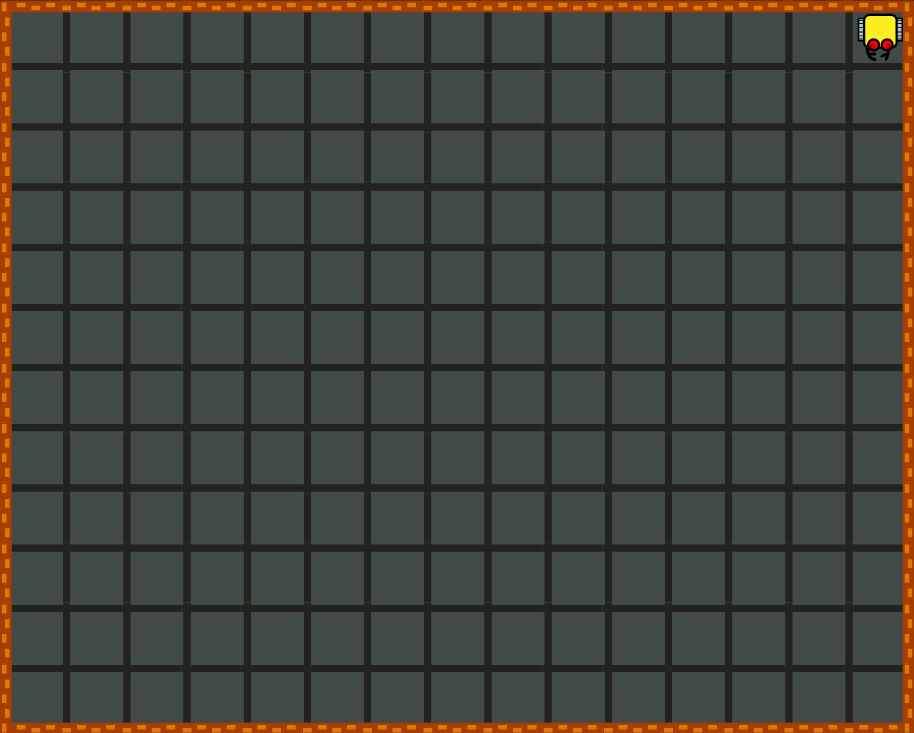
\includegraphics[width=14cm]{img/binomial.png}
\vspace{-0mm}
\caption{Karel is ready for the statistical experiment.}
%\vspace{-1cm}
\label{fig:binomial}
\end{center}
\end{figure}

\noindent
He has many gems in his bag -- at least 100 but 500 is better. His task is to 
descend towards the South wall of the maze, put a gem on the ground, and 
return to his starting position. Before descending to the next row, however, he 
always throws a coin and either goes straight south or diagonally south-west. 
Since he descends 11 rows, the probablity that he makes it to the south-east
corner of the maze is the same as throwing the coin 11 times and getting 
always heads. Mathematically, this is $1/2$ to the power of $11$, which translates 
into $0.0488$ \%. This is also the probability that he goes 11 times south-west.
He repeats this experiment until his bag is empty.
Here is the corresponding code:\\

\begin{bbox}
\begin{Verbatim}[commandchars=\\\{\}]
\PY{c}{\PYZsh{} Return to upper right corner and}
\PY{c}{\PYZsh{} face South:}
\PY{k}{def} GoCorner
  \PY{k}{while} \PY{n+nb+bp}{not} \PY{n+nb+bp}{north}
    \PY{n+nf}{left}
  \PY{n+nf}{right}
  \PY{k}{while} \PY{n+nb+bp}{not} \PY{n+nb+bp}{wall}
    \PY{n+nf}{go}
  \PY{n+nf}{left}
  \PY{k}{repeat} 11
    \PY{n+nf}{go}
  \PY{n+nf}{right}
  \PY{n+nf}{right}

\PY{c}{\PYZsh{} Descend one row towards the South.}
\PY{c}{\PYZsh{} Either go straight or to the right:}
\PY{k}{def} Move
  \PY{k}{if} \PY{n+nb+bp}{rand}
    \PY{n+nf}{go}
  \PY{k}{else}
    \PY{n+nf}{right}
    \PY{n+nf}{go}
    \PY{n+nf}{left}
    \PY{n+nf}{go}

\PY{c}{\PYZsh{} Descend towards the South wall}
\PY{c}{\PYZsh{} and drop a gem:}
\PY{k}{while} \PY{n+nb+bp}{not} \PY{n+nb+bp}{empty}
  \PY{k}{repeat} 11
    \PY{n}{Move}
\PY{n+nf}{put}
\PY{n}{GoCorner}

\end{Verbatim}
\end{bbox}
\vspace{6mm}
\hfill

\newpage
\noindent
You can download this project from NCLab's public database.
Fig. \ref{fig:binomial2} shows the result. The distribution of the 
gems along the South wall approximate the binomial distribution. 

\begin{figure}[!ht]
\begin{center}

\includegraphics[width=14cm]{img/binomial2.png}
\vspace{-0mm}
\caption{Distribution of gems along the South wall when Karel is done.}
%\vspace{-1cm}
\label{fig:binomial2}
\end{center}
\end{figure}

\noindent
Credit for this example goes to Ed Keppelmann from UNR. 

%%%%%%%%%%%%%%%%%%%%%%%%%%%%%%%%%%%%%%%%%%%%%%%%%%%%%%%%%%%%%%%%%%%%%%%%%%%%%%%

\section{Recursion} \label{sec:recursion}

\subsection{\ \ Objectives} 
 
\begin{itemize}
\item Understand what recursion is and when it can be useful.
\item Learn to write good recursive algorithms.
\end{itemize}
By a {\em recursive} algorithm we mean an algorithm that makes a call to itself. How does it sound?
In our life we use recursion all the time, without noticing it. For example, when we descend 
a staircase, our algorithm is:\\

\begin{bbox}
\begin{Verbatim}[commandchars=\\\{\}]
Descend_staircase
    Descend_one_step
    If this_was_not_the_last_step
        Descend_staircase
\end{Verbatim}
\end{bbox}
\vspace{6mm}

\noindent
Recursion is not applicable to all types of problems, but it can be very 
helpful, especially for problems where we can
\begin{itemize}
\item reduce the problem to a similar one which is smaller in size, 
\item apply the same algorithm to the smaller problem. 
\end{itemize}
In the program, this means that some command calls itself, either 
directly or through other commands.

\subsection[\ \ How it works]{How it works} 

Consider the following Karel program:\\

\begin{bbox}
\begin{Verbatim}[commandchars=\\\{\}]
\PY{k}{def} reach_wall
    \PY{k}{if} \PY{n+nb+bp}{not} \PY{n+nb+bp}{wall}
        \PY{n+nf}{go}
        reach_wall

reach_wall
\end{Verbatim}
\end{bbox}
\vspace{6mm}

\noindent
Imagine that the initial position of the robot is like in Fig. \ref{fig:rec1}.


\begin{figure}[!ht]
\begin{center}
\includegraphics[width=6cm]{img/rec-1.png}
\end{center}
\vspace{-4mm}
\caption{Robot's initial position.}
\label{fig:rec1}
\vspace{-4mm}
\end{figure}
\noindent
When the command {\tt reach\_wall} is first called, the robot stands three steps away from the wall and 
thus the {\tt if not wall} condition passes. Then the command {\tt go} follows and the robot's 
position changes as shown in Fig. \ref{fig:rec2}. 

\begin{figure}[!ht]
\begin{center}
\includegraphics[width=6cm]{img/rec-2.png}
\end{center}
\vspace{-4mm}
\caption{Robot's position after making the first step forward.}
\label{fig:rec2}
\vspace{-4mm}
\end{figure}
\noindent
Next the robot executes the {\tt reach\_wall} command that follows the {\tt go} command. A good way to 
understand what happens is to imagine that the command is replaced with its own body. So the corresponding 
code would look as follows:\\

\begin{bbox}
\begin{Verbatim}[commandchars=\\\{\}]
\PY{k}{if} \PY{n+nb+bp}{not} \PY{n+nb+bp}{wall}
    \PY{n+nf}{go}
    \PY{k}{if} \PY{n+nb+bp}{not} \PY{n+nb+bp}{wall}
        \PY{n+nf}{go}
        reach_wall
\end{Verbatim}
\end{bbox}
\vspace{6mm}

\noindent
Since the robot is two steps away from the wall, the second {\tt if not wall} condition passes and 
he makes a second step forward. His new position is shown in Fig. \ref{fig:rec3}.

\begin{figure}[!ht]
\begin{center}
\includegraphics[width=6cm]{img/rec-3.png}
\end{center}
\vspace{-4mm}
\caption{Robot's position after making the second step forward.}
\label{fig:rec3}
\vspace{-4mm}
\end{figure}
\noindent
Next the robot executes the third {\tt reach\_wall} command. Again we can imagine that the command 
is replaced with its own body. The corresponding code would look as follows:\\

\begin{bbox}
\begin{Verbatim}[commandchars=\\\{\}]
\PY{k}{if} \PY{n+nb+bp}{not} \PY{n+nb+bp}{wall}
    \PY{n+nf}{go}
    \PY{k}{if} \PY{n+nb+bp}{not} \PY{n+nb+bp}{wall}
        \PY{n+nf}{go}
        \PY{k}{if} \PY{n+nb+bp}{not} \PY{n+nb+bp}{wall}
            \PY{n+nf}{go}
            reach_wall
\end{Verbatim}
\end{bbox}
\vspace{6mm}

\noindent
Since the robot is one step away from the wall, the third {\tt if not wall} condition passes and 
he makes a third step forward. His new position is shown in Fig. \ref{fig:rec4}.
\newpage

\begin{figure}[!ht]
\begin{center}
\includegraphics[width=6cm]{img/rec-4.png}
\end{center}
\vspace{-4mm}
\caption{Robot's position after making the third step forward.}
\label{fig:rec4}
%\vspace{-10mm}
\end{figure}
\noindent
Now the robot stands in front of the wall, so it gets more interesting. The 
{\tt reach\_wall} command is executed one more time, so we can imagine that its body 
is pasted into the code one last time:\\

\begin{bbox}
\begin{Verbatim}[commandchars=\\\{\}]
\PY{k}{if} \PY{n+nb+bp}{not} \PY{n+nb+bp}{wall}
    \PY{n+nf}{go}
    \PY{k}{if} \PY{n+nb+bp}{not} \PY{n+nb+bp}{wall}
        \PY{n+nf}{go}
        \PY{k}{if} \PY{n+nb+bp}{not} \PY{n+nb+bp}{wall}
            \PY{n+nf}{go}
            \PY{k}{if} \PY{n+nb+bp}{not} \PY{n+nb+bp}{wall}
                \PY{n+nf}{go}
                reach_wall
\end{Verbatim}
\end{bbox}
\vspace{6mm}

\noindent
However, now the {\tt if not wall} condition does not pass, which means that  
the program is finished!

\subsection[\ \ The base case]{The base case}

In the last example we have observed one important fact: To prevent infinite recursion, we 
used an {\tt if} statement. The {\tt else} statement was omitted which meant "else do nothing".
In recursive algorithms, we always need an {\tt if} or {\tt if-else} statement of some sort, 
where one branch makes a recursive call while the other one does not. 
The branch without a recursive call is called the {\em base case}. A bad example 
of a recursive command without a base case would be\\

\begin{bbox}
\begin{Verbatim}[commandchars=\\\{\}]
\PY{k}{def} left_forever
    \PY{n+nf}{left}
    left_forever
\end{Verbatim}
\end{bbox}
\vspace{6mm}

\noindent
This program is an infinite recursion that needs to be stopped using the 
red stop button.

\subsection[\ \ When should recursion be used?]{When should recursion be used?}

The recursive command {\tt reach\_wall} that we defined above may not be the most useful example 
since the same functionality could be achieved more elegantly without recursion, just with\\

\begin{bbox}
\begin{Verbatim}[commandchars=\\\{\}]
\PY{k}{def} reach_wall
    \PY{k}{while} \PY{n+nb+bp}{not} \PY{n+nb+bp}{wall}
        \PY{n+nf}{go}
\end{Verbatim}
\end{bbox}
\vspace{6mm}

\noindent
If there is a small task that needs to be solved repeatedly in order to get a bigger task done,
then often one can write both a non-recursive and recursive version. Recall for example the Diamond
Staircase example from Section \ref{sec:newcom}. The small task there was to climb one step and pick 
up the gem, ending up facing east. A non-recursive version of the algorithm would be:\\

\begin{bbox}
\begin{Verbatim}[commandchars=\\\{\}]
\PY{k}{def} climb_one_step
    \PY{n+nf}{left}
    \PY{n+nf}{go}
    \PY{n+nf}{right}
    \PY{n+nf}{go}
    \PY{n+nf}{get}

\PY{k}{while} \PY{n+nb+bp}{not} \PY{n+nb+bp}{home}
    climb_one_step
\end{Verbatim}
\end{bbox}
\vspace{6mm}

\noindent
A recursive version of the same:\\

\begin{bbox}
\begin{Verbatim}[commandchars=\\\{\}]
\PY{k}{def} climb_the_stairs
    \PY{k}{if} \PY{n+nb+bp}{not} \PY{n+nb+bp}{home}
        \PY{n+nf}{left}
        \PY{n+nf}{go}
        \PY{n+nf}{right}
        \PY{n+nf}{go}
        \PY{n+nf}{get}
        climb_the_stairs

climb_the_stairs
\end{Verbatim}
\end{bbox}
\vspace{6mm}

\noindent
If an algorithm comes in both a recursive and a non-recursive version, then the following 
should be taken into account:
\begin{itemize}
\item The recursive version will be slightly slower than a non-recursive one. The reason is 
      the overhead related to creating a new instance of the recursive command and calling it. 
\item The recursive version will also require more memory -- when a recursive command is called 
      1000 times, then it actually exists in 1000 copies in the memory. Hence, recursion is 
      not recommended with very large numbers of repetitions.
\end{itemize}
Recursive algorithms are used mainly where non-recursive ones are cumbersome to design. 
For example, much code written for traversing tree-like data structures is recursive. Also certain 
sorting algorithms are more naturally written in recursive form. We will discuss these subjects 
in more detail later.

\subsection[\ \ Mutually recursive commands]{Mutually recursive commands}

Recursion can have interesting forms. For example, there can be a pair of commands
that call themselves mutually, such as the commands {\tt odd} and 
{\tt even} in the following example (that also solves the Diamond Staircase
problem). Note the presence of base case in both recursive commands:\\
 
\begin{bbox}
\begin{Verbatim}[commandchars=\\\{\}]
\PY{k}{def} climb_step
    \PY{n+nf}{left}
    \PY{n+nf}{go}
    \PY{n+nf}{right}
    \PY{n+nf}{go}
    \PY{n+nf}{get} 

\PY{k}{def} odd
    \PY{k}{if} not home
        climb_step
        even

\PY{k}{def} even
    \PY{k}{if} not home
        climb_step
        odd
    
odd
\end{Verbatim}
\end{bbox}

%%%%%%%%%%%%%%%%%%%%%%%%%%%%%%%%%%%%%%%%%%%%%%%%%%%%%%%%%%%%%%%%%%%%%%%%%%%%%%%

\section{Appendix - Overview of Functionality by Mode}\label{sec:newfunc3}

\subsection[\ \ Manual mode (Section \ref{sec:manual})]{Manual mode (Section \ref{sec:manual})}

In Manual mode, Karel can be guided by clicking on buttons:
\begin{itemize}
\item Go ... make one step forward.
\item Left ... turn left.
\item Right ... turn right.
\item Put ... put a gem on the ground.
\item Get ... pick up a gem from the ground.
\end{itemize}

\subsection[\ \ Programming mode 1 (Sections \ref{sec:bridge} -- \ref{sec:repeat})]{Programming mode 1 (Sections \ref{sec:bridge} -- \ref{sec:repeat})}

In Programming mode 1, Karel can be guided by typing the commands:
\begin{itemize}
\item {\tt go} ... make one step forward.
\item {\tt left} ... turn left.
\item {\tt right} ... turn right.
\item {\tt put} ... put a gem on the ground.
\item {\tt get} ... pick up a gem from the ground.
\item {\tt repeat} ... counting loop (repeat an action a given number of times).
\end{itemize}

\subsection[\ \ Programming mode 2 (Sections \ref{sec:cond} -- \ref{sec:recursion})]{Programming mode 2 (Sections \ref{sec:cond} -- \ref{sec:recursion})}

New commands:
\begin{itemize}
\item {\tt if - else} ... condition.
\item {\tt while} ... conditional loop (repeat an action while a condition is satisfied).
\item {\tt def} ... define a new command.
\end{itemize}
Additional new keywords:
\begin{itemize}
\item {\tt wall} ... sensor that checks True if the robot faces a wall.
\item {\tt gem} ... sensor that checks True if there is a gem within the robot's reach.
\item {\tt empty} ... sensor that checks True if the robot's bag with gems is empty.
\item {\tt home} ... sensor that checks True if the robot is at home.
\item {\tt north} ... sensor that checks True if the robot faces North.
\end{itemize}
New functionality:
\begin{itemize}
\item Recursion (a command can make a call to itself).
\end{itemize}

\subsection[\ \ Programming mode 3 (Sections \ref{sec:var}, \ref{sec:logic})]{Programming mode 3 (Sections \ref{sec:var}, \ref{sec:logic})}

New keywords:
\begin{itemize}
\item {\tt print} ... print strings and variables.
\item {\tt gpsx} ... GPS coordinate in the horizontal direction.
\item {\tt gpsy} ... GPS coordinate in the vertical direction.
\item {\tt a = 0} ... create a new variable {\tt a} and initialize it with zero (or another 
      integer number).\\ For additional ways to initialize variables see Subsection \ref{par:var}.
\item {\tt inc(a)} ... increases the value of variable {\tt a} by one.
\item {\tt inc(a, value)} ... increases the value of variable {\tt a} by {\tt value}.
\item {\tt dec(a)} ... decreases the value of variable {\tt a} by one.
\item {\tt dec(a, value)} ... decreases the value of variable {\tt a} by {\tt value}.
\item {\tt rand} ... random command (returns randomly {\tt True} or {\tt False}).
\item {\tt return} ... returns a value, to be used in functions.
\item {\tt and} ... binary logical {\em and}.
\item {\tt or} ... binary logical {\em or}.
\item {\tt not} ... unary logical {\em not}.
\item {\tt L[]} ... create an empty list {\tt L}.
\item {\tt len(L)} ... length of list {\tt L}.
\item {\tt L[i]} ... object at position {\tt i} in list {\tt L}. Note: {\tt L[0]} is the first item in the list.
\item {\tt L.append(x)} ... appends {\tt x} to the end of list {\tt L}.
\item {\tt x = L.pop()} ... removes the last item of list {\tt L} and assigns it to {\tt x}.
\item {\tt del L[i]} ... removes from list {\tt L} object at position {\tt i}. 
\end{itemize}
New functionality:
\begin{itemize}
\item Numerical and logical (Boolean) variables.
\item Complex logical expressions.
\item Functions that return values.
\item Lists.
\end{itemize}

\section{What next?}

Congratulations, you made it through Karel the Robot! We hope that you 
enjoyed the textbook and exercises. If you can think of any way to 
improve the application Karel the Robot or this textbook, we would like
to hear from you. If you have an interesting new game or exercise for 
Karel, please let us know as well. \\

\noindent
You are now ready to dive into a next programming language! We would 
recommend Python which is a modern dynamic programming 
language that is used in many applications in business, science,
engineering, and other areas.\\

\noindent
In any case, our team wishes you good luck, and keep us in your 
favorite bookmarks! \\

\hbox{} \hfill{} Your Authors


